\documentclass[12pt,dvipsnames]{exam}
\usepackage[utf8]{inputenc}
\usepackage{setspace}
\usepackage{float}
\spacing{1.5}
\usepackage{graphicx}
\usepackage{braket}
\usepackage{physics}
\usepackage{tcolorbox}
\tcbuselibrary{theorems}
\usepackage{mathrsfs}
\usepackage[colorlinks=true, urlcolor=blue]{hyperref}
\usepackage[margin=1in]{geometry}
\usepackage{amsmath,amssymb}
\usepackage{multicol}
\usepackage[spanish]{babel}
\usepackage{graphicx}% Include figure files
\usepackage{bm}% bold math
\usepackage{caption}
\usepackage{xcolor}
\usepackage{color}
\usepackage{listings}
\usepackage{cancel}
\usepackage{fancyhdr}
\usepackage{capt-of}
%\newcommand{\class}{Física Teórica I - R. Depine}
%\newcommand{\term}{FCEyN - 2do Cuatrimestre 2017}
\usepackage[usenames]{color}
\usepackage{amsmath}
 
\newcommand{\commentedbox}[2]{%
  \mbox{
    \begin{tabular}[t]{@{}c@{}}
    $\boxed{\displaystyle#1}$\\
    #2
    \end{tabular}%
  }%
}



\pagestyle{head}
\firstpageheader{}{}{}
\runningheader{\class}{\examnum Pág. \thepage\ de \numpages}{\examdate}
\runningheadrule

\begin{document}

\renewcommand{\figurename}{Fig.}

	\title{Experimentos con las ecuaciones de aguas poco profundas (SWE) para los casos de ondas de gravedad, de Kelvin y de Rossby y su aplicación para la explicación del fenómeno de El Niño.} \vspace{-2ex}}
	\author{Reto Reynal, Juan \hspace{0.2cm} \href{https://github.com/jrr1984/SWE_2D}{LINK}: https://github.com/jrr1984/SWE\_2D\\
		\textsc{\small Estructura de la materia 1 - Departamento de Física - FCEyN, UBA}\\
	\textsc{\small Profesor: Fernando Minotti}\\
	\\ \date{}
	}
	\maketitle
	
	
	\newpage
	\thispagestyle{empty} 
\tableofcontents
\newpage

\section{Modelo matemático: Ecuaciones de aguas poco profundas}
Las ecuaciones de aguas poco profundas en 2D, en inglés: \textit{shallow water equations} (en adelante, SWE), son ecuaciones de conservación del volumen y del momento total en cada dirección, en particular de $h$, $uh$, $vh$ respectivamente que, en forma de flujo, tienen las siguientes expresiones:

\begin{equation}
\tcboxmath[colback=blue!25!white,colframe=blue, title=Ec. de Continuidad:]{
    \frac{\partial h}{\partial t} + \frac{\partial (u h)}{\partial x} + \frac{\partial (v h)}{\partial y} = 0 }
\end{equation}

\begin{equation}
\tcboxmath{\frac{\partial u h}{\partial t} + \frac{\partial (u^{2} h + g h^{2}/2)}{\partial x} + \frac{\partial (u v h)}{\partial y} = h \left(f v - g \frac{\partial H}{\partial x}\right)}
\label{cons1}
\end{equation}

\begin{equation}
\tcboxmath{    \frac{\partial v h}{\partial t} + \frac{\partial (u v h)}{\partial x} + \frac{\partial (v^{2} h + g h^{2}/2)}{\partial y}  = h \left(-f u - g \frac{\partial H}{\partial y}\right)}
\label{cons2}
\end{equation}

donde $\vec{u} = (u,v,0)^{t}$ es el vector velocidad que podría ser del viento ó del agua en el océano, $\vec{\Omega} = (0,0,f)^{t}$ es la velocidad angular de rotación de la tierra de donde se desprende que $f$ es el parámetro de Coriolis y g es el módulo de la aceleración gravitatoria terrestre. El parámetro de Coriolis es modelado a partir de una variación lineal en la coordenada $y$ del tipo: $f = f_{0} + \beta (y - \overline{y})$. Entonces $f = f_{0}$ se encuentra en la mitad del dominio en la dirección de la coordenada $y$; $\overline{y}$ es el valor medio de la coordenada y. El gradiente de presión fue puesto junto a las derivadas parciales espaciales del lado izquierdo (en adelante, LHS).

\begin{figure}[H]
\centering
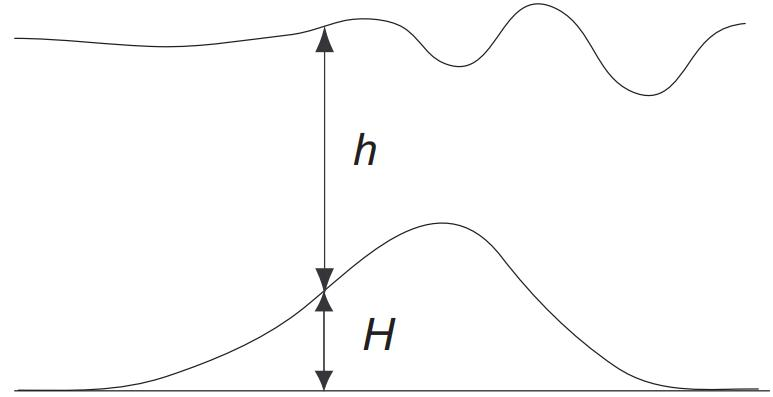
\includegraphics[scale=0.7]{s1.jpeg}
\caption{Esquema del escenario modelado, donde $h$ es la profundidad del fluido y H es la altura de la orografía.} \label{f1}
\end{figure}

\section{Esquema numérico elegido: Lax-Wendroff}

El esquema numérico elegido que va a ser integrado en el tiempo es el de Lax-Wendroff. Es un método de 2do orden tanto el tiempo como en el espacio pues el error de truncado es de orden $\mathcal{O}({\Delta t}^{2} + {\Delta x}^{2} + {\Delta y}^{2})$. En este sentido y además por su estabilidad, es una propuesta superadora al esquema de Lax-Friedrichs que es un método de 1er orden de exactitud.

A continuación se copia un cuadro con un resumen de las ecuaciones diferenciales del modelo a la izquierda (Ecs. de Continuidad, \ref{cons1} y \ref{cons2}) y de las ecuaciones discretizadas con el esquema de Lax-Wendroff a la derecha (Ecs. \ref{esq1}, \ref{esq2}, \ref{esq3} y \ref{esq4}). Todas las derivaciones de las ecuaciones del cuadro se encuentran en los apéndices.

\begin{figure}[H]
\centering
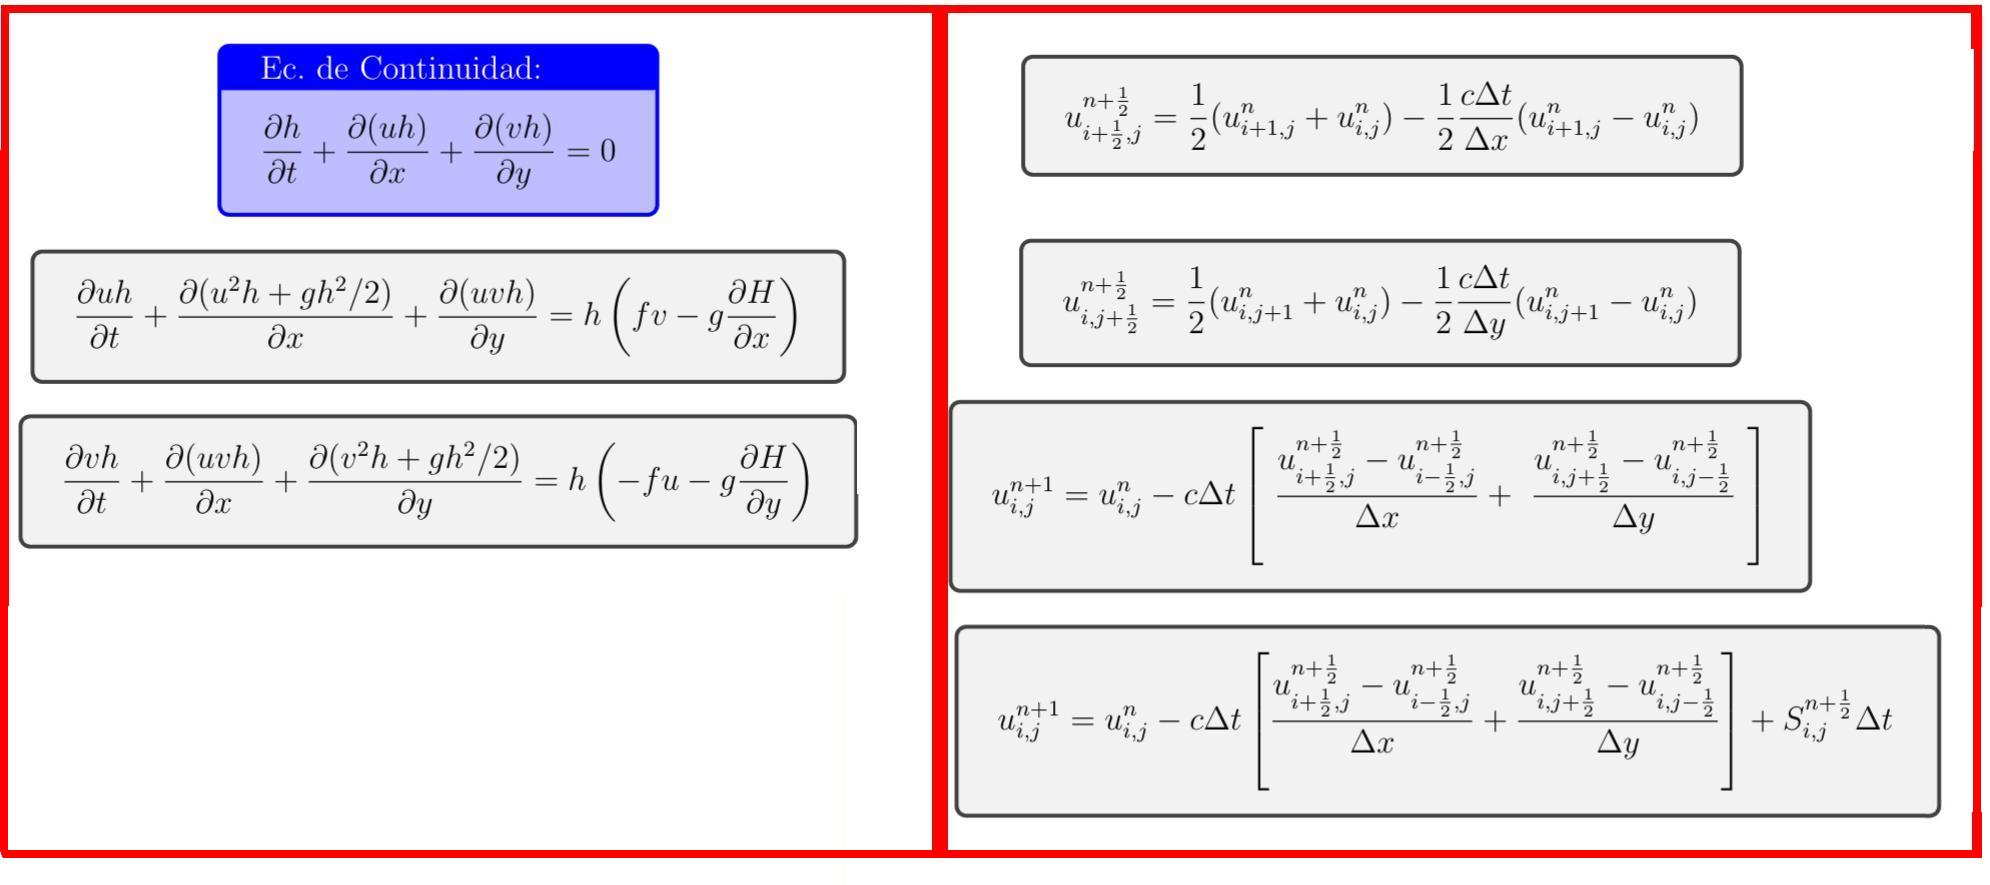
\includegraphics[scale=0.35]{reseqs.jpeg}
\caption{Resumen de las ecuaciones diferenciales del modelo a la izquierda y de las ecuaciones discretizadas con el esquema de Lax-Wendroff a la derecha.} \label{reqs}
\end{figure}

Si ahora hacemos los siguientes reemplazos para reexpresar convenientemente las ecuaciones diferenciales:
\begin{equation*}
UH = u h
\end{equation*}

\begin{equation*}
VH = v h
\end{equation*}

\begin{equation*}
UX = hu^{2} + gh^{2}/2
\end{equation*}


\begin{equation*}
UY = uvh \text{, en la ecuación del momento de $u$}
\end{equation*}

\begin{equation*}
VX = uvh \text{, en la ecuación del momento de $v$}
\end{equation*}

\begin{equation*}
VY = hv^2+\frac{1}{2}gh^2
\end{equation*}

\begin{equation*}
SX = hfv - gh\dfrac{\partial H}{\partial x}
\end{equation*}

\begin{equation*}
SY = -hfu - gh\dfrac{\partial H}{\partial y}
\end{equation*}


De esta manera las SWE quedan de la siguiente manera:

\begin{equation}
    \tcboxmath[]{\dfrac{\partial UH}{\partial t} + \dfrac{\partial UX}{\partial x} + \dfrac{\partial UY}{\partial y} =SX}
    \label{s1}
\end{equation}
    
\begin{equation}
\tcboxmath[]{\dfrac{\partial VH}{\partial t} + \dfrac{\partial VX}{\partial x} + \dfrac{\partial VY}{\partial y} =SY} 
\label{s2}
\end{equation}

\begin{equation}
\tcboxmath[]{\dfrac{\partial h}{\partial t} + \dfrac{\partial UH}{\partial x} + \dfrac{\partial VH}{\partial y} = 0}}
\label{s3}
\end{equation}

Finalmente, lo que hay que hacer es ahora discretizar estas ecuaciones con el esquema de Lax-Wendroff que tenemos ya resuelto para este tipo de ecuaciones. Por un lado, las de convección en 2D con un término fuente/sumidero, discretización dada por la Ec. \ref{esq4},  como es el caso de \ref{s1}, \ref{s2} y por otro lado, la de 2D de convección común \ref{s3} cuya discretización viene dada por la Ec. \ref{esq3}.

A continuación se muestran como quedan discretizadas las soluciones con el esquema de Lax-Wendroff:

\begin{equation*}
    h_{i,j}^{n+1} = h_{i,j}^n - \dfrac{\Delta t}{\Delta x} \left( UH_{i+\frac{1}{2},j}^{n+\frac{1}{2}} - UH_{i-\frac{1}{2},j}^{n+\frac{1}{2}}   \right) - \dfrac{\Delta t}{\Delta y} \left( VH_{i,j+\frac{1}{2}}^{n+\frac{1}{2}} - VH_{i,j-\frac{1}{2}}^{n+\frac{1}{2}} \right) 
\end{equation*}

\begin{equation*}
    UH_{i,j}^{n+1} = UH_{i,j}^n - \dfrac{\Delta t}{\Delta x} \left( UX_{i+\frac{1}{2},j}^{n+\frac{1}{2}} - UX_{i-\frac{1}{2},j}^{n+\frac{1}{2}}   \right) - \dfrac{\Delta t}{\Delta y} \left( UY_{i,j+\frac{1}{2}}^{n+\frac{1}{2}} - UY_{i,j-\frac{1}{2}}^{n+\frac{1}{2}} \right) + \Delta t SX_{i,j}^{n+\frac{1}{2}}
\end{equation*}

\begin{equation*}
    
VH_{i,j}^{n+1} = VH_{i,j}^n - \dfrac{\Delta t}{\Delta x} \left( VX_{i+\frac{1}{2},j}^{n+\frac{1}{2}} - VX_{i-\frac{1}{2},j}^{n+\frac{1}{2}}   \right) - \dfrac{\Delta t}{\Delta y} \left( VY_{i,j+\frac{1}{2}}^{n+\frac{1}{2}} - VY_{i,j-\frac{1}{2}}^{n+\frac{1}{2}} \right) + \Delta t SY_{i,j}^{n+\frac{1}{2}}
\end{equation*}


\subsection{Condiciones de contorno}

En cuanto a las condiciones de contorno, se pueden simular diferentes escenarios dependiendo el fenómeno que se quiera estudiar. Las condiciones de contorno son condiciones de borde pues especifican qué es lo que ocurre en los extremos de la región que se estudia que puede ser desde una simple pileta de natación a una cierta porción del océano donde se toma una distancia latitudinal mucho mayor que la meridional.

Ejemplos de condiciones de contorno:
\begin{enumerate}
    \item Condición de borde de no-dezlizamiento (no-slip): u y v son nulas en los bordes, es decir: $u(1,y) = u(end,y) = v(x,1) = v(x,end) = 0$
    \item Reflectivas: 
    
    $u(1,y) = -u(2,y)$
    
    $u(end,y) = - u(end-1,y)$ 
    
    $v(x,1) = -v(x,2)$
    
    $v(x,end) = - v(x,end-1)$
    
La velocidad en los bordes es la contraria a la velocidad del punto más cercano al mismo que es la velocidad con la que se aproxima al borde.

\item Bordes libres, no ejercen ninguna influencia sobre el fluido. Simplemente se adjudica a los bordes la velocidad del vecino más cercano en la malla.

$u(1,y) = u(2,y) , u(end,y) = u(end-1,y)$

$v(x,1) = v(x,2) , v(x,end) = v(x,end-1)$


\item Periódicas: lo que ocurre en uno de los dos extremos, ocurre también en el otro.

$u(1,y) = u(end,y)$


$v(x,1) = v(x,end)$

\end{enumerate}
 A continuación se muestran los experimentos realizados con la simulación, se hace notar que hay una infinidad de experimentos posibles dado la variedad de condiciones de contorno y de las condiciones iniciales que se pueden dar como perturbación del fluido.
 
\subsection{Aproximaciones del plano f y del plano $\beta$}

El hecho de que la Tierra sea esférica no resulta fundamental para los modelos implementados por lo que es conveniente tratar las ecuaciones con coordenadas cartesianas en lugar de coordenadas esféricas como sería natural.


La aproximación del plano f tiene un rango de validez limitado. Sólo aplica a movimientos de escala muy pequeña comparada con el radio de la Tierra (6371 km) y lejos del ecuador.

En el plano f la rotación es considerada constante pero en la atmósfera real y en el océano la componente vertical de la rotación de la Tierra varía con la latitud de la siguiente forma:

\begin{equation*}
    f = 2 \Omega sin(\phi)
\end{equation*}

Consideremos ahora el plano $\beta$ que se muestra en la Fig. \ref{bee}. El plano indicado es tangencial a la superficie terrestre y en ese plano se puede considerar que el parámetro $f$ varía linealmente con la latitud. Haciendo una expansión de Taylor de $f$ alrededor de una latitud $\phi_{0}$, en $y=0$, se obtiene:

\begin{equation*}
    f(y) = f(0) + \frac{d f}{d y } \rvert_{\phi_{0}} y = f_{0} + \beta y
\end{equation*}
donde $f_{0} = 2 \Omega sin(\phi)$ y $\beta = 2 \Omega cos(\phi_{0})/R_{T}$ donde $R_{T} = 6371 km$ es el radio de la Tierra.

\begin{figure}[H]
\centering
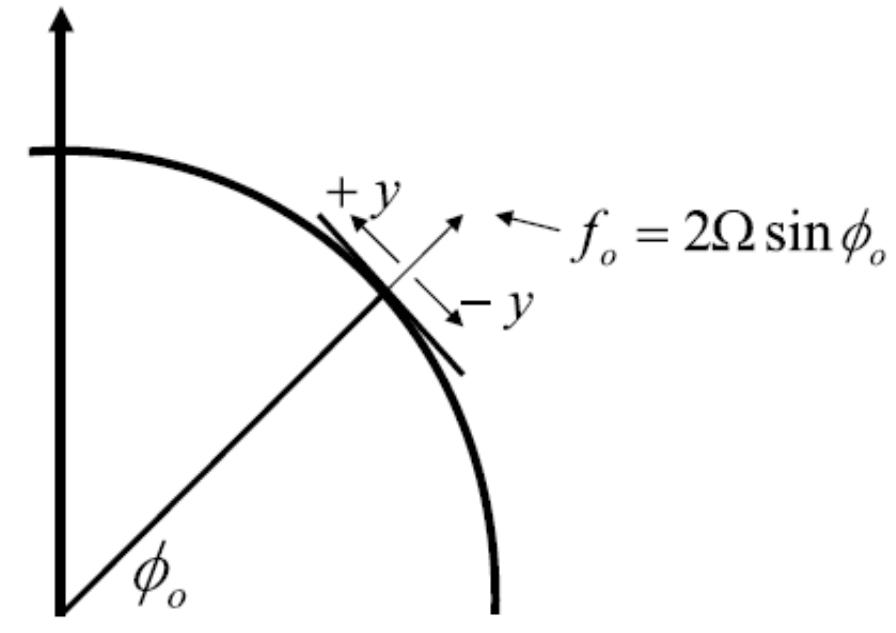
\includegraphics[scale=0.4]{bet.jpeg}
\caption{Esquema de la aproximación del plano $\beta$}
\label{bee}
\end{figure}


La aproximación del plano $\beta$ es válida para movimientos de escala comparable al radio de la Tierra lejos de los polos, y vale incluso en el ecuador donde $f_{0}=0$. Dicha aproximación tiene en cuenta los efectos dinámicos más importantes que hay que considerar por la esfericidad de la Tierra pero sin tener en cuenta algunos efectos geométricos que pueden ser complicados de resolver y no son esenciales para describir los fenómenos aquí estudiados.

Es importante notar las aproximaciones del plano f y del plano $\beta$ son muy útiles, ya que partiendo de un problema cuyas coordenadas naturales son las coordenadas esféricas, nos permiten trabajar más fácilmente con expresiones más simples y tratables en cartesianas.

\section{Experimentos}

El código, videos, imágenes se encuentra separado por tipo de experimento \href{https://github.com/jrr1984/SWE_2D}{aquí}. 

Link: \textit{https://github.com/jrr1984/SWE\_2D}
\subsection{Ondas de gravedad}

Las ondas de gravedad puras son las ondas más simples modeladas por las SWE que pueden ser generadas a partir de especificar las condiciones iniciales que consisten en dar una altura inicial no uniforme del fluido como perturbación en algún punto de la región superficial que se analiza. En particular, se puede dar como condición inicial una especie de 'gota de fluido' con una forma funcional del tipo gaussiana en algún área del dominio del fluido, posición que puede ser elegida corriendo la gaussiana (tanto en x como en y); con el campo de velocidades $\vec{u}$ en reposo. Como estamos en el caso de un fluido no rotante, el parámetro de Coriolis $f$ es nulo. Por último, la superficie sólida sobre la que se apoya el fluido es plana, $H$ no presenta irregularidades. Esto es:

\begin{equation*}
    u_{t=0} = v_{t=0} = 0
\end{equation*}


\begin{equation*}
    f = 0 \hspace{0.5cm} \text{pues} \hspace{0.5cm} f_{0} = \beta = 0
\end{equation*}

\begin{equation*}
    H(x,y) = 0
\end{equation*}

A continuación se realiza una explicación del fenómeno de las ondas gravitatorias a partir de la simulación realizada que consiste en realizar la evolución temporal de las SWE en una cierta porción del océano. Inicialmente se genera una perturbación del tipo gaussiana como se explicó \texttt{ut supra} que sería como una ola inicial que hace mover a una cierta porción del agua cercana.

De esta manera, en el primer frame de la simulación, inicialmente sólo se ve la perturbación que comienza para el \texttt{contour plot} de h pero el campo de velocidades es nulo (el color verde en la escala indica el valor 0 tanto para $u$ como para $v$). Es decir, se cumplen las condiciones iniciales: 


1) Campo de velocidades nulo inicialmente:

\begin{figure}[H]
\centering
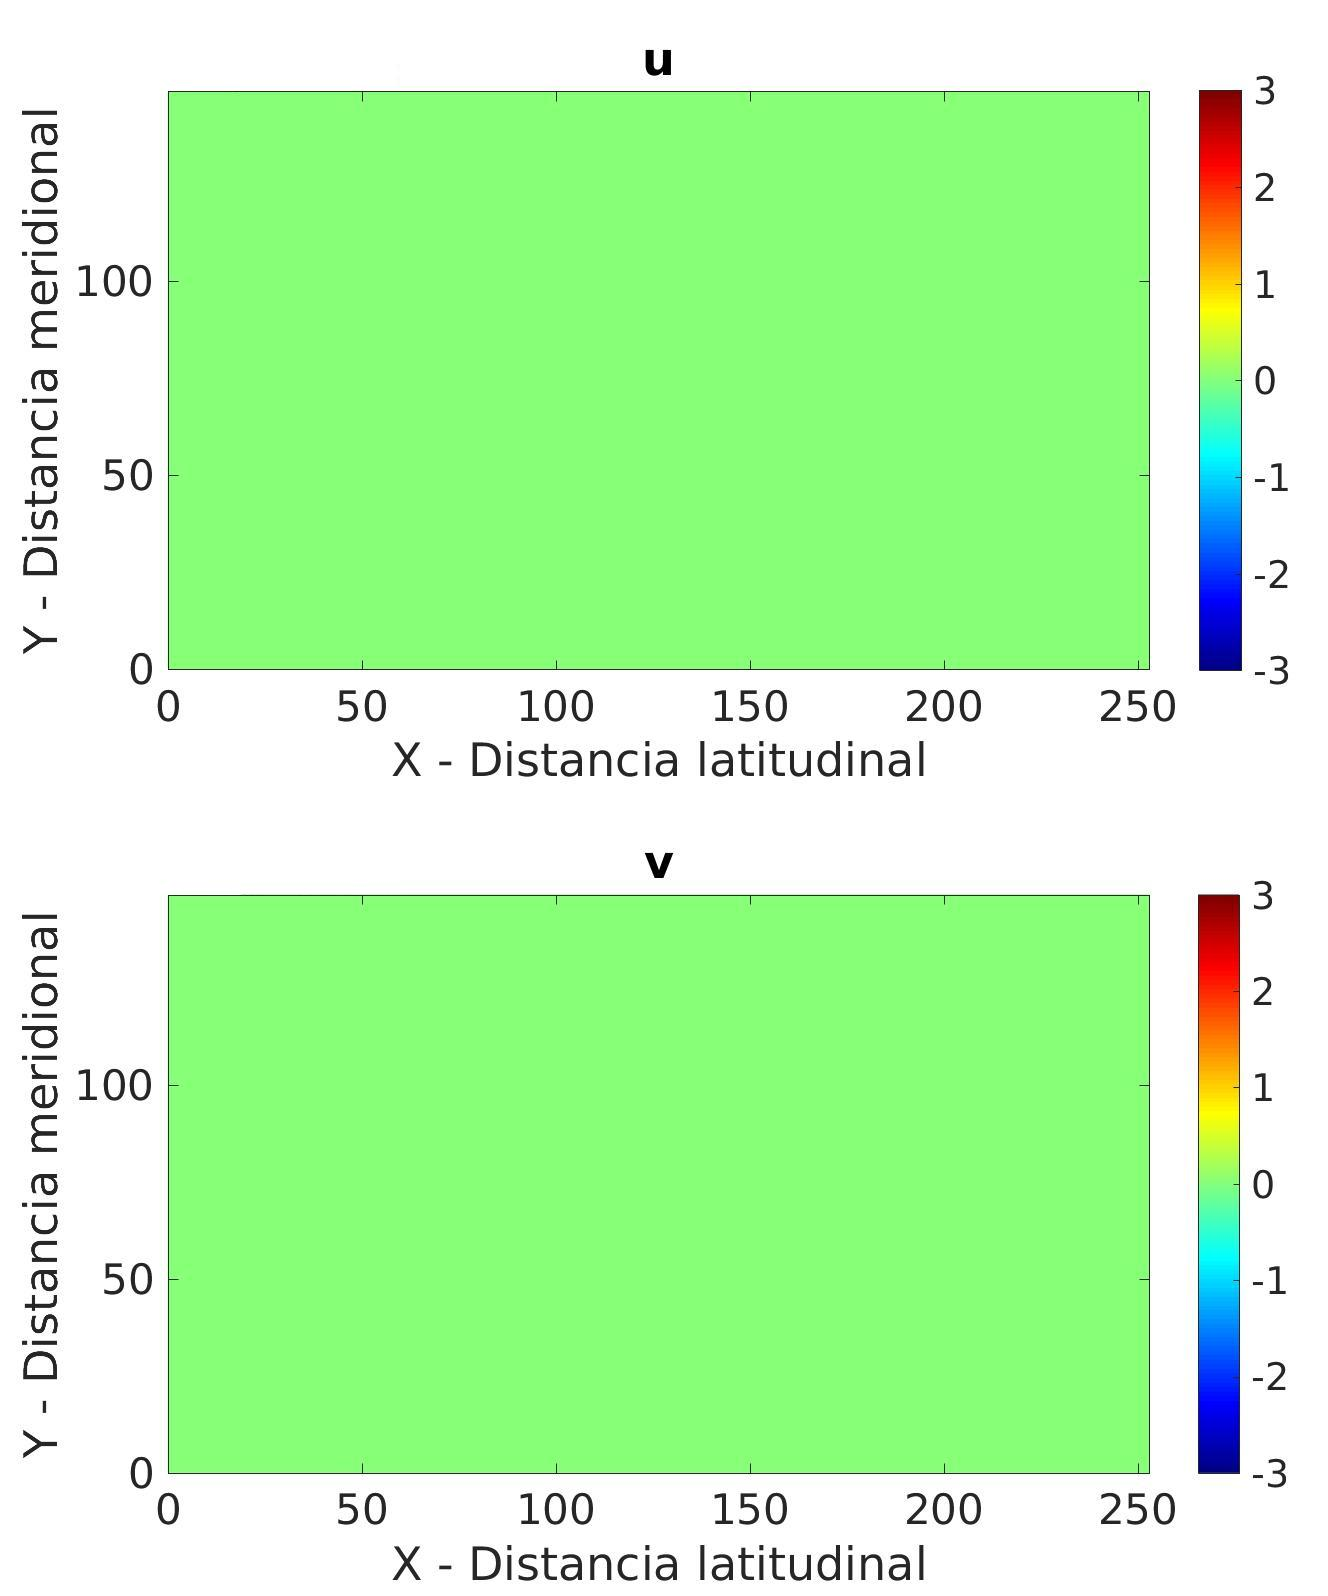
\includegraphics[scale=0.4]{uv0.jpeg}
\caption{Gráficos tipo mapa de contorno en colores para las velocidades $u$ y $v$ en el dominio x-y.}
\end{figure}

2) Perturbación gaussiana en el punto elegido del dominio, no se observa el campo de velocidades todavía graficado. En azul se muestra todo el dominio que no se encuentra perturbado todavía, mientras que en rojo y en colores escalados tendiendo al celeste como se muestra en la barra de colores se muestra la perturbación.

\begin{figure}[H]
\centering
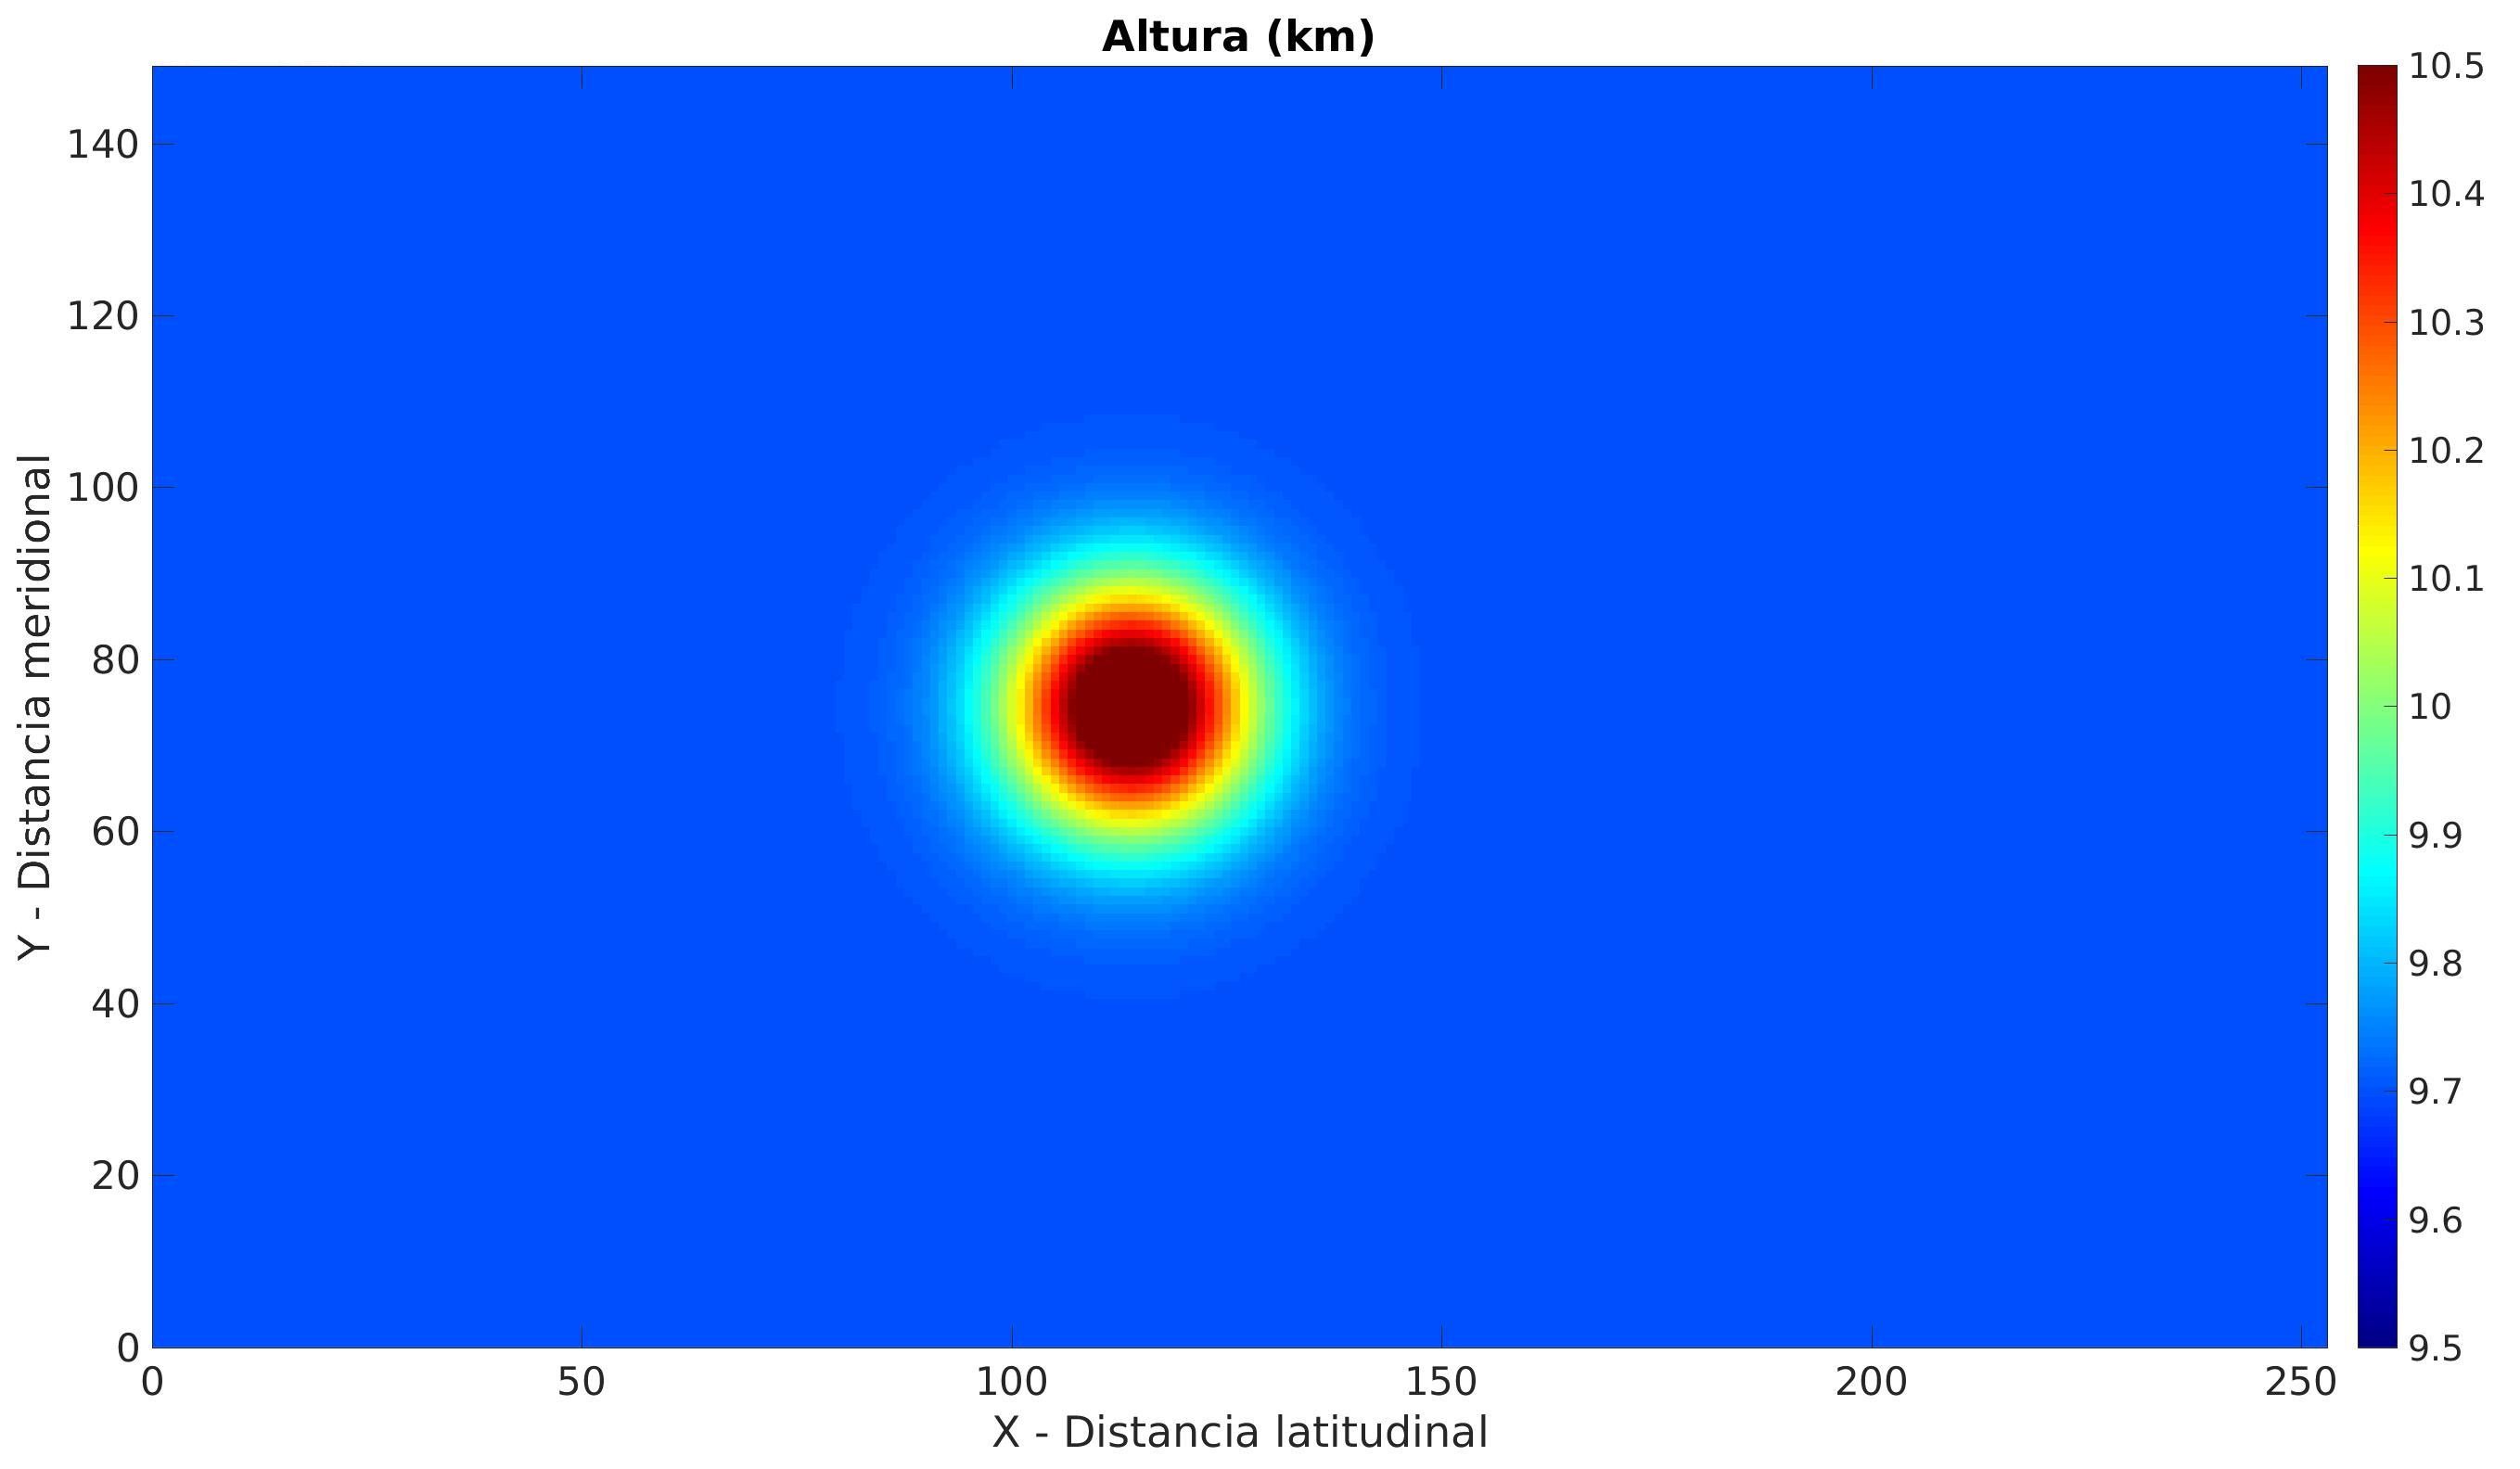
\includegraphics[scale=0.3]{h0.jpeg}
\caption{Gráfico tipo mapa de contorno en colores para la altura $h$ en el dominio x-y. }
\end{figure}


A medida que la simulación va iterando en el tiempo las velocidades $u$ y $v$ van siendo inducidas en el dominio del fluido estudiado y lo que se ven son ondas que son irradiadas radialmente hacia afuera.% con velocidad de fase $ c = \sqrt{g h}$

\begin{figure}[H]
\begin{minipage}[b]{0.5\linewidth} 
\centering
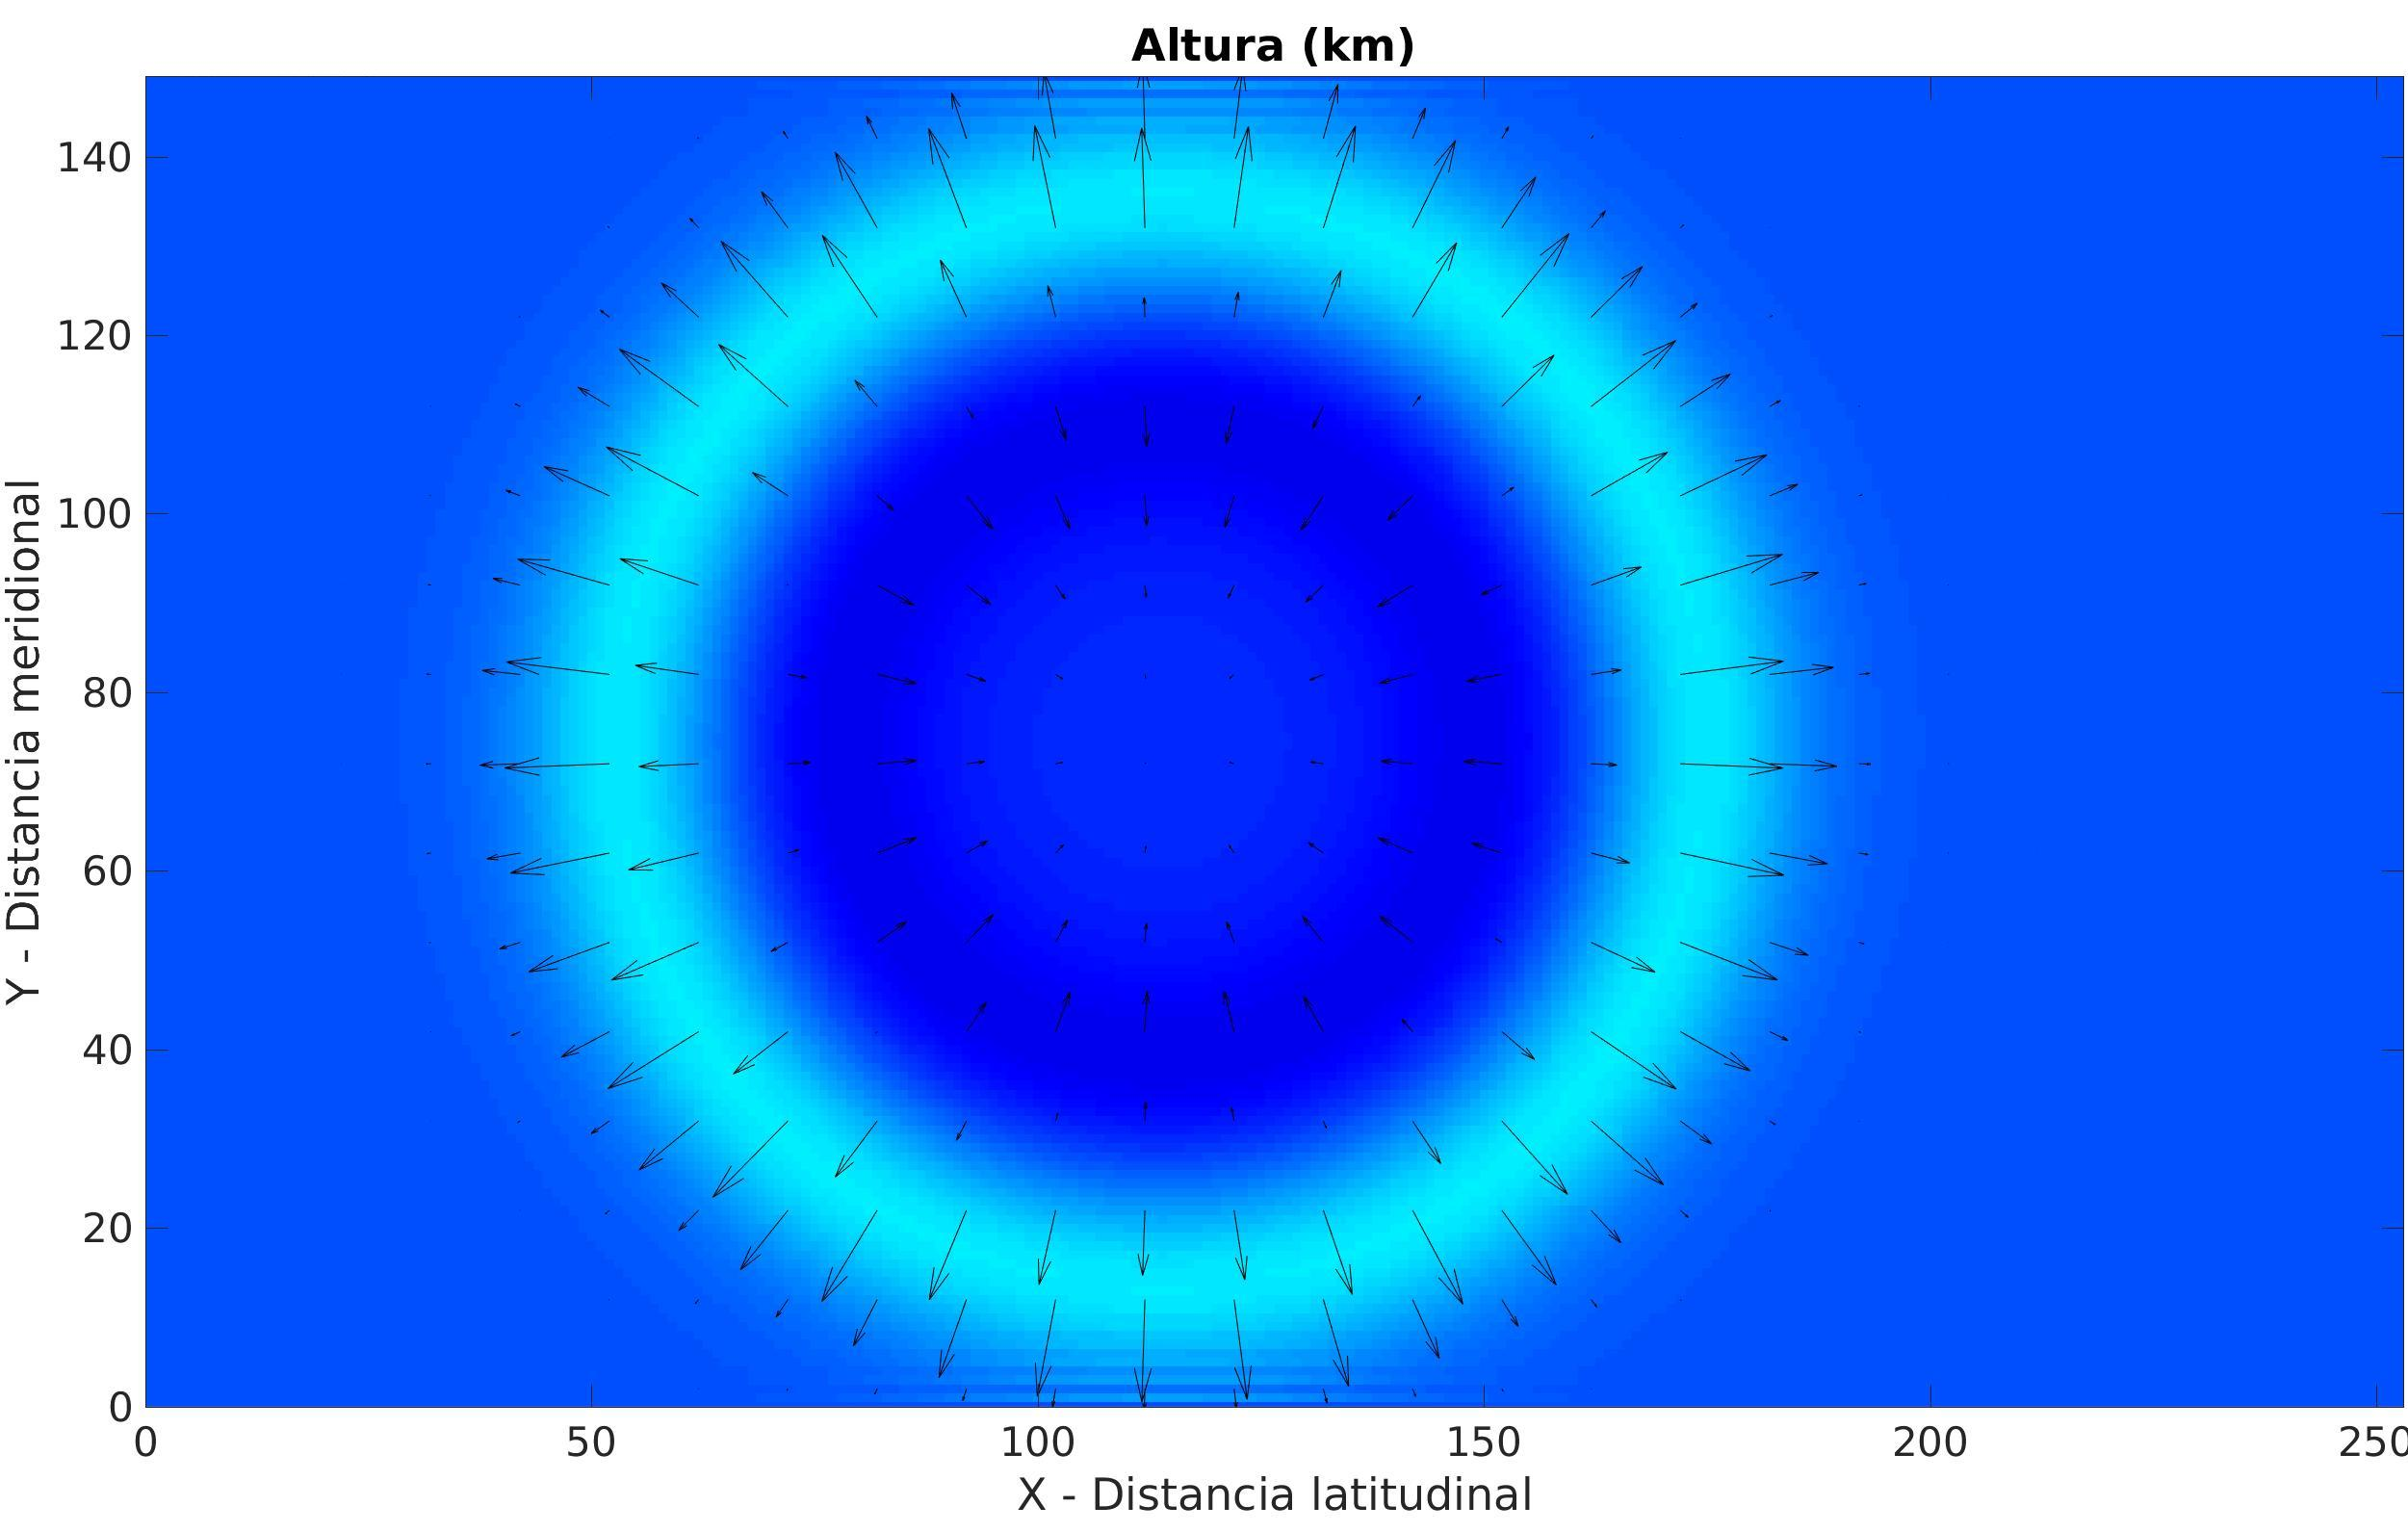
\includegraphics[scale=0.2]{hd.jpeg}
\caption{ }
\end{minipage}
\hspace{0.1cm} 
\begin{minipage}[b]{0.5\linewidth}
\centering
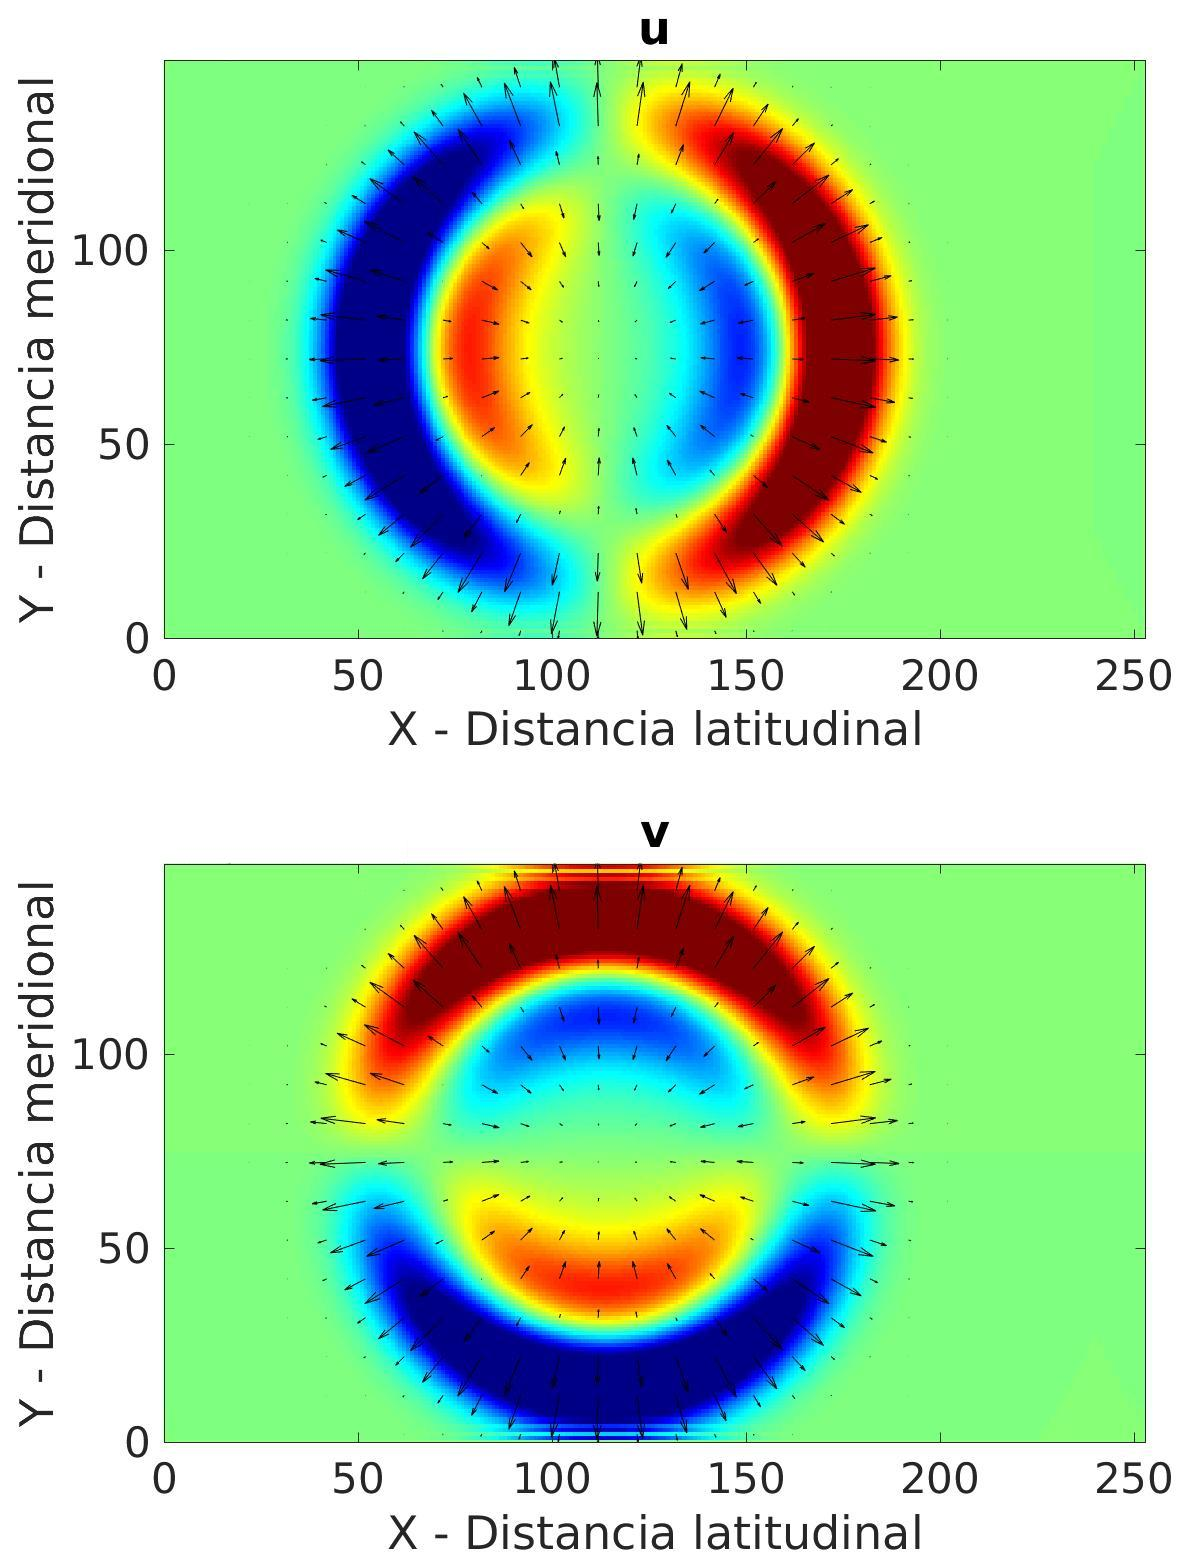
\includegraphics[scale=0.35]{uvd.jpeg}
\caption{}
\end{minipage}
\end{figure}

Simulaciones completas tipo película:
\begin{itemize}
    \item \href{https://www.youtube.com/watch?v=orZdrxbf_gk&list=PLO4Ke9LzSkdFyMJ0r6OuJdeCk4Ys-RJ3t&index=1}{Altura - Ondas de gravedad.}
    \item \href{https://www.youtube.com/watch?v=rBKvAQhE7c0&list=PLO4Ke9LzSkdFyMJ0r6OuJdeCk4Ys-RJ3t&index=2}{Campo de velocidades - Ondas de gravedad.}
\end{itemize}

Si se quiere ver el efecto de las condiciones de borde, se deben elegir los parámetros correctos: duración de la simulación, ancho de la malla en x e y, etc.

Las ondas de gravedad no presentan prácticamente vorticidad, para todo tiempo de la simulación, como se puede ver en el siguiente \texttt{contour plot}:


\begin{figure}[H]
\centering
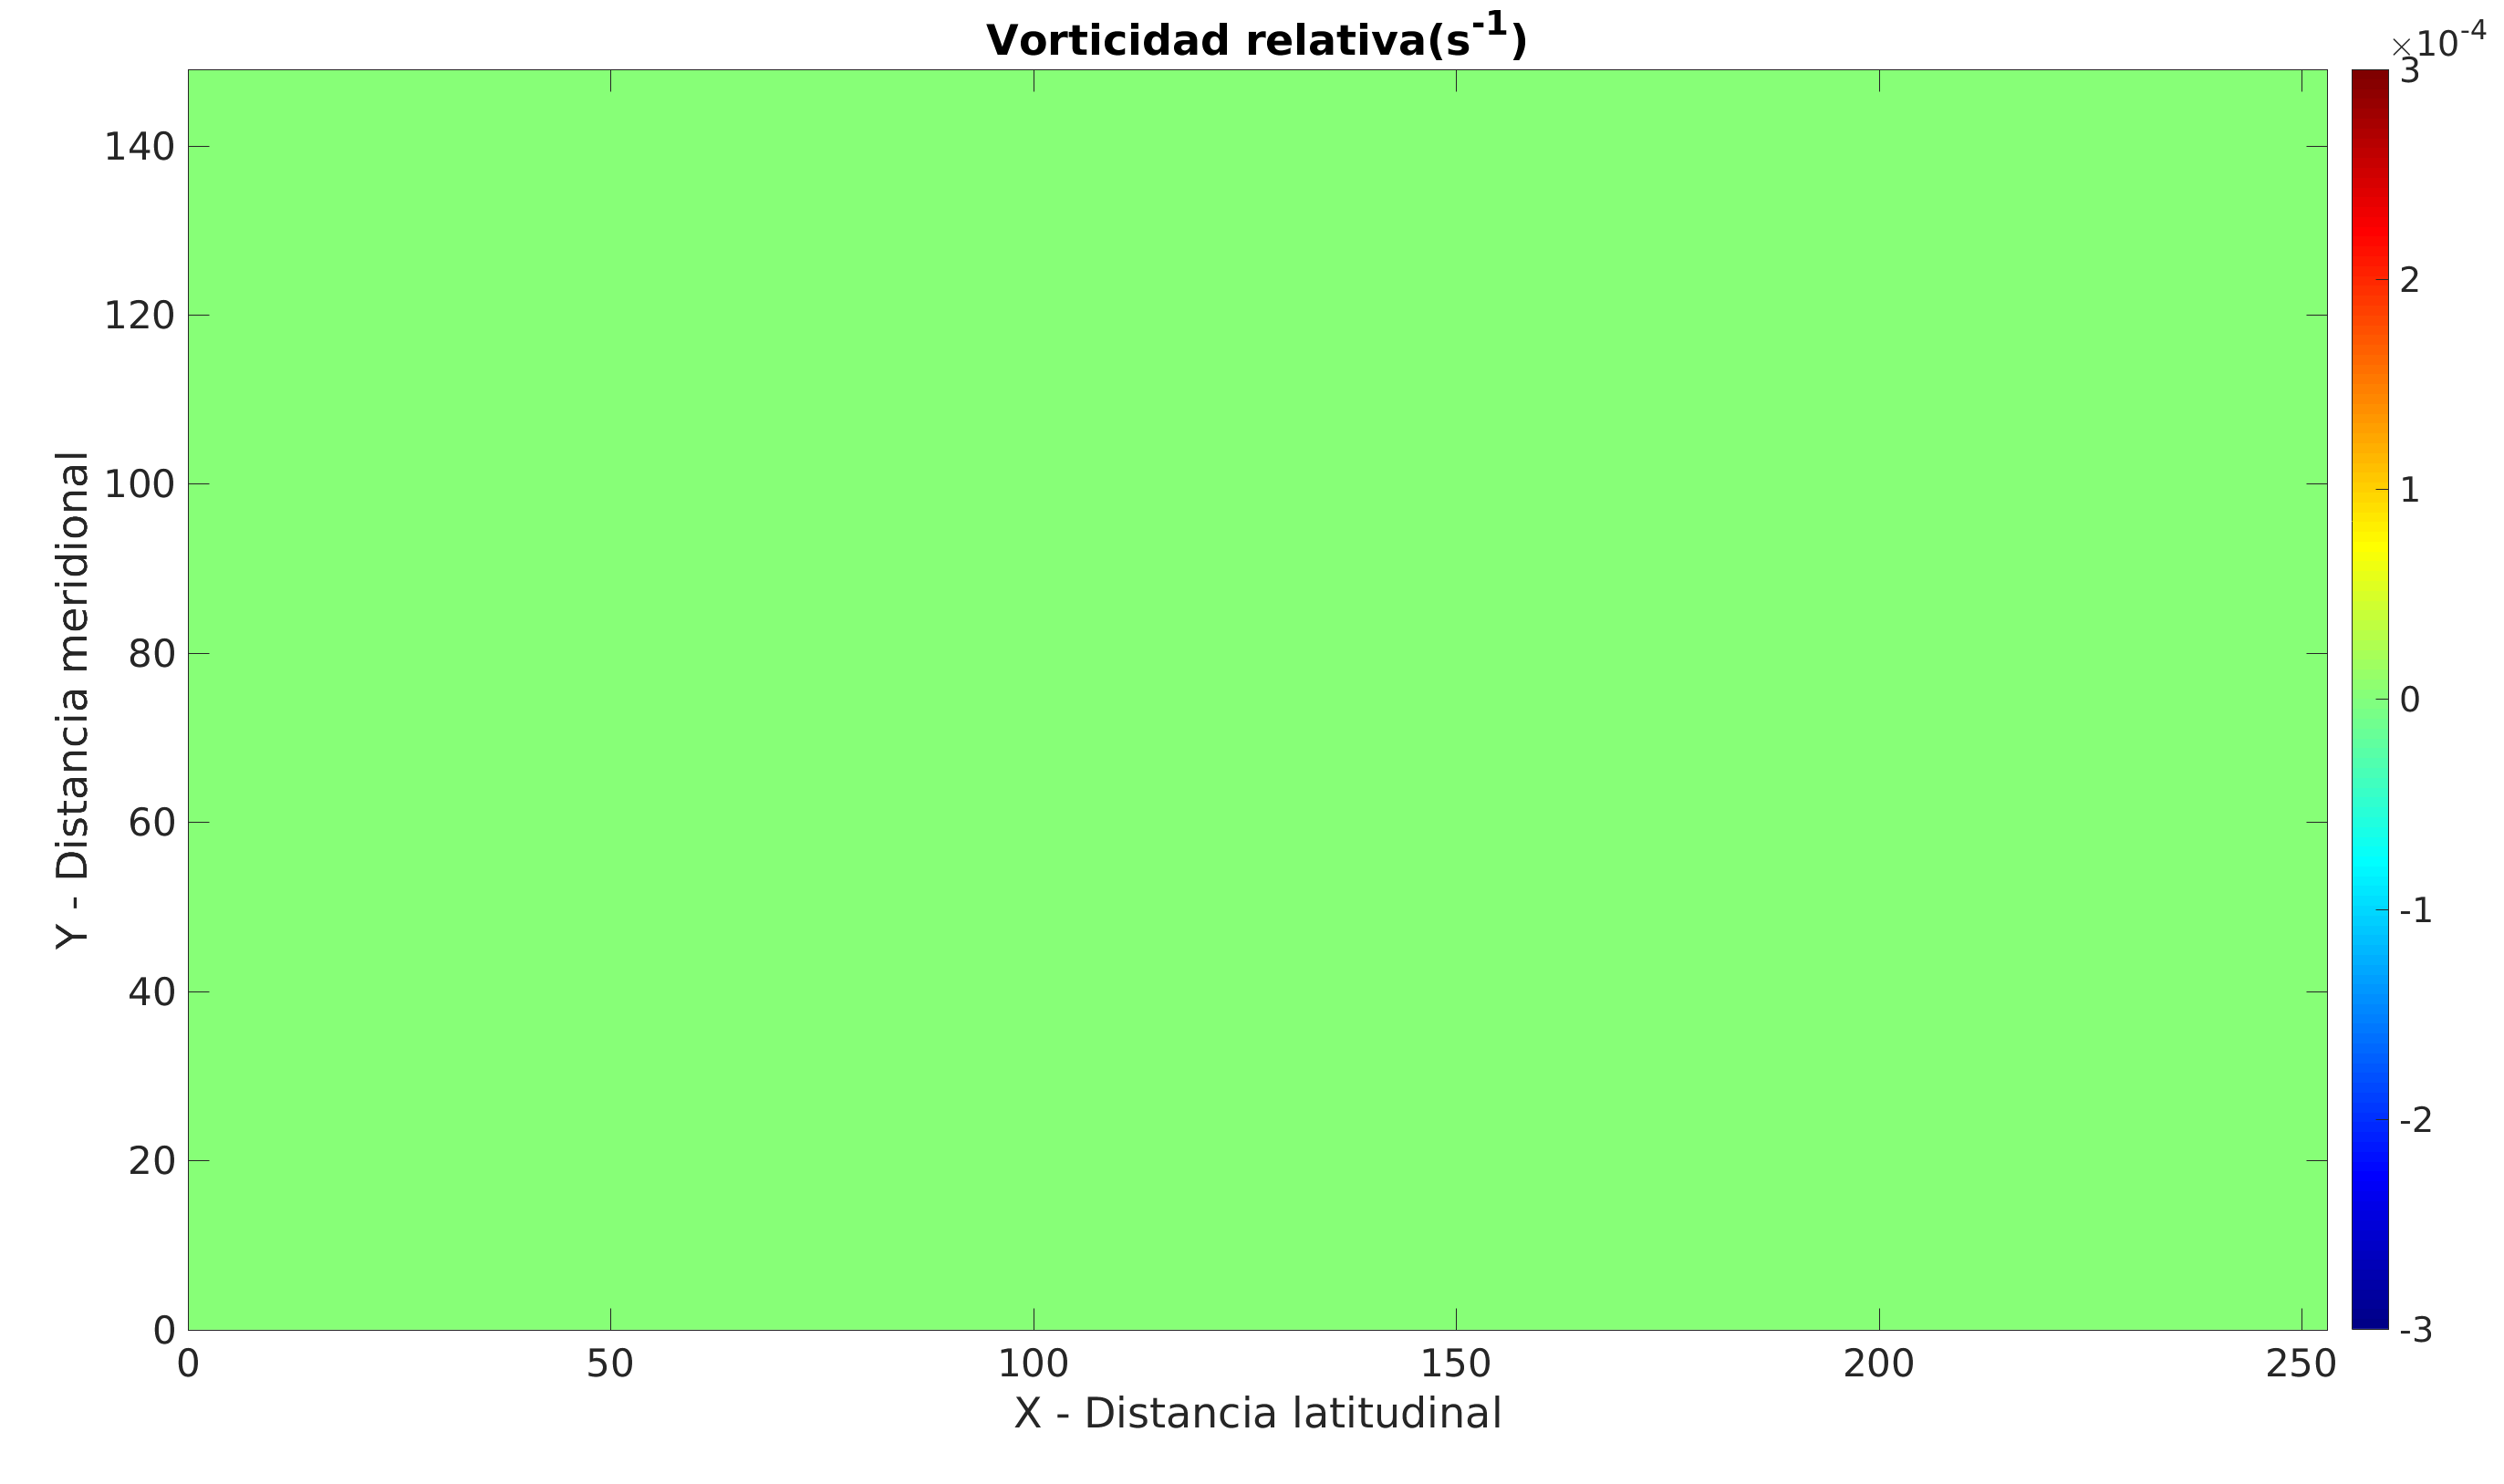
\includegraphics[scale=0.35]{vort1.png}
\caption{Gráfico tipo mapa de contorno para la vorticidad en el dominio x-y.}
\label{vort_g}
\end{figure}

El gráfico de contorno es prácticamente de color verde claro en todo el dominio, color que indica el valor nulo de la vorticidad. Esto se debe a que el término de Coriolis $f$ vale cero en este caso. Entonces se puede decir que el fluido no rota como era de esperar pues la única interaccción que tiene el fluido es gravitatoria.

\subsection{Ondas ecuatoriales de Kelvin}

Las ondas ecuatoriales de Kelvin son un tipo de ondas oceánicas 'atrapadas' en el ecuador. Son un tipo de ondas de gravedad pero ahora con el término de Coriolis $f$ prendido: es decir, se considera a la fuerza de Coriolis y esto se debe a que la onda viaja lo suficientemente lento como para que haya que considerar sus efectos.

Se tienen las mismas condiciones iniciales que para las ondas de gravedad y el fondo también es considerado plano.


\begin{equation*}
    u_{t=0} = v_{t=0} = 0
\end{equation*}


\begin{equation*}
    H(x,y) = 0
\end{equation*}


El parámetro de Coriolis ahora es:

\begin{equation*}
    f_{0} = 0 ,  \text{lo que indica que las ondas se propagan en el ecuador.}
\end{equation*}

\begin{equation*}
    \beta = 5 . 10^{-10} m^{-1} s^{-1} , \text{lo suficientemente grande como para mostrar el efecto de Coriolis.} $\xrightarrow{}$ Estabilidad de la simulación es muy sensible a dicho parámetro.
\end{equation*}

La perturbación gaussiana inicial en el dominio del fluido se puede ver en la Fig. \ref{k1}. Dicha perturbación se va propagando longitudinalmente a lo largo del ecuador y se forma una onda de Kelvin en dirección hacia el este de mayor intensidad como se puede ver en la Fig. \ref{k2}.

\begin{figure}[H]
\begin{minipage}[b]{0.5\linewidth} 
\centering
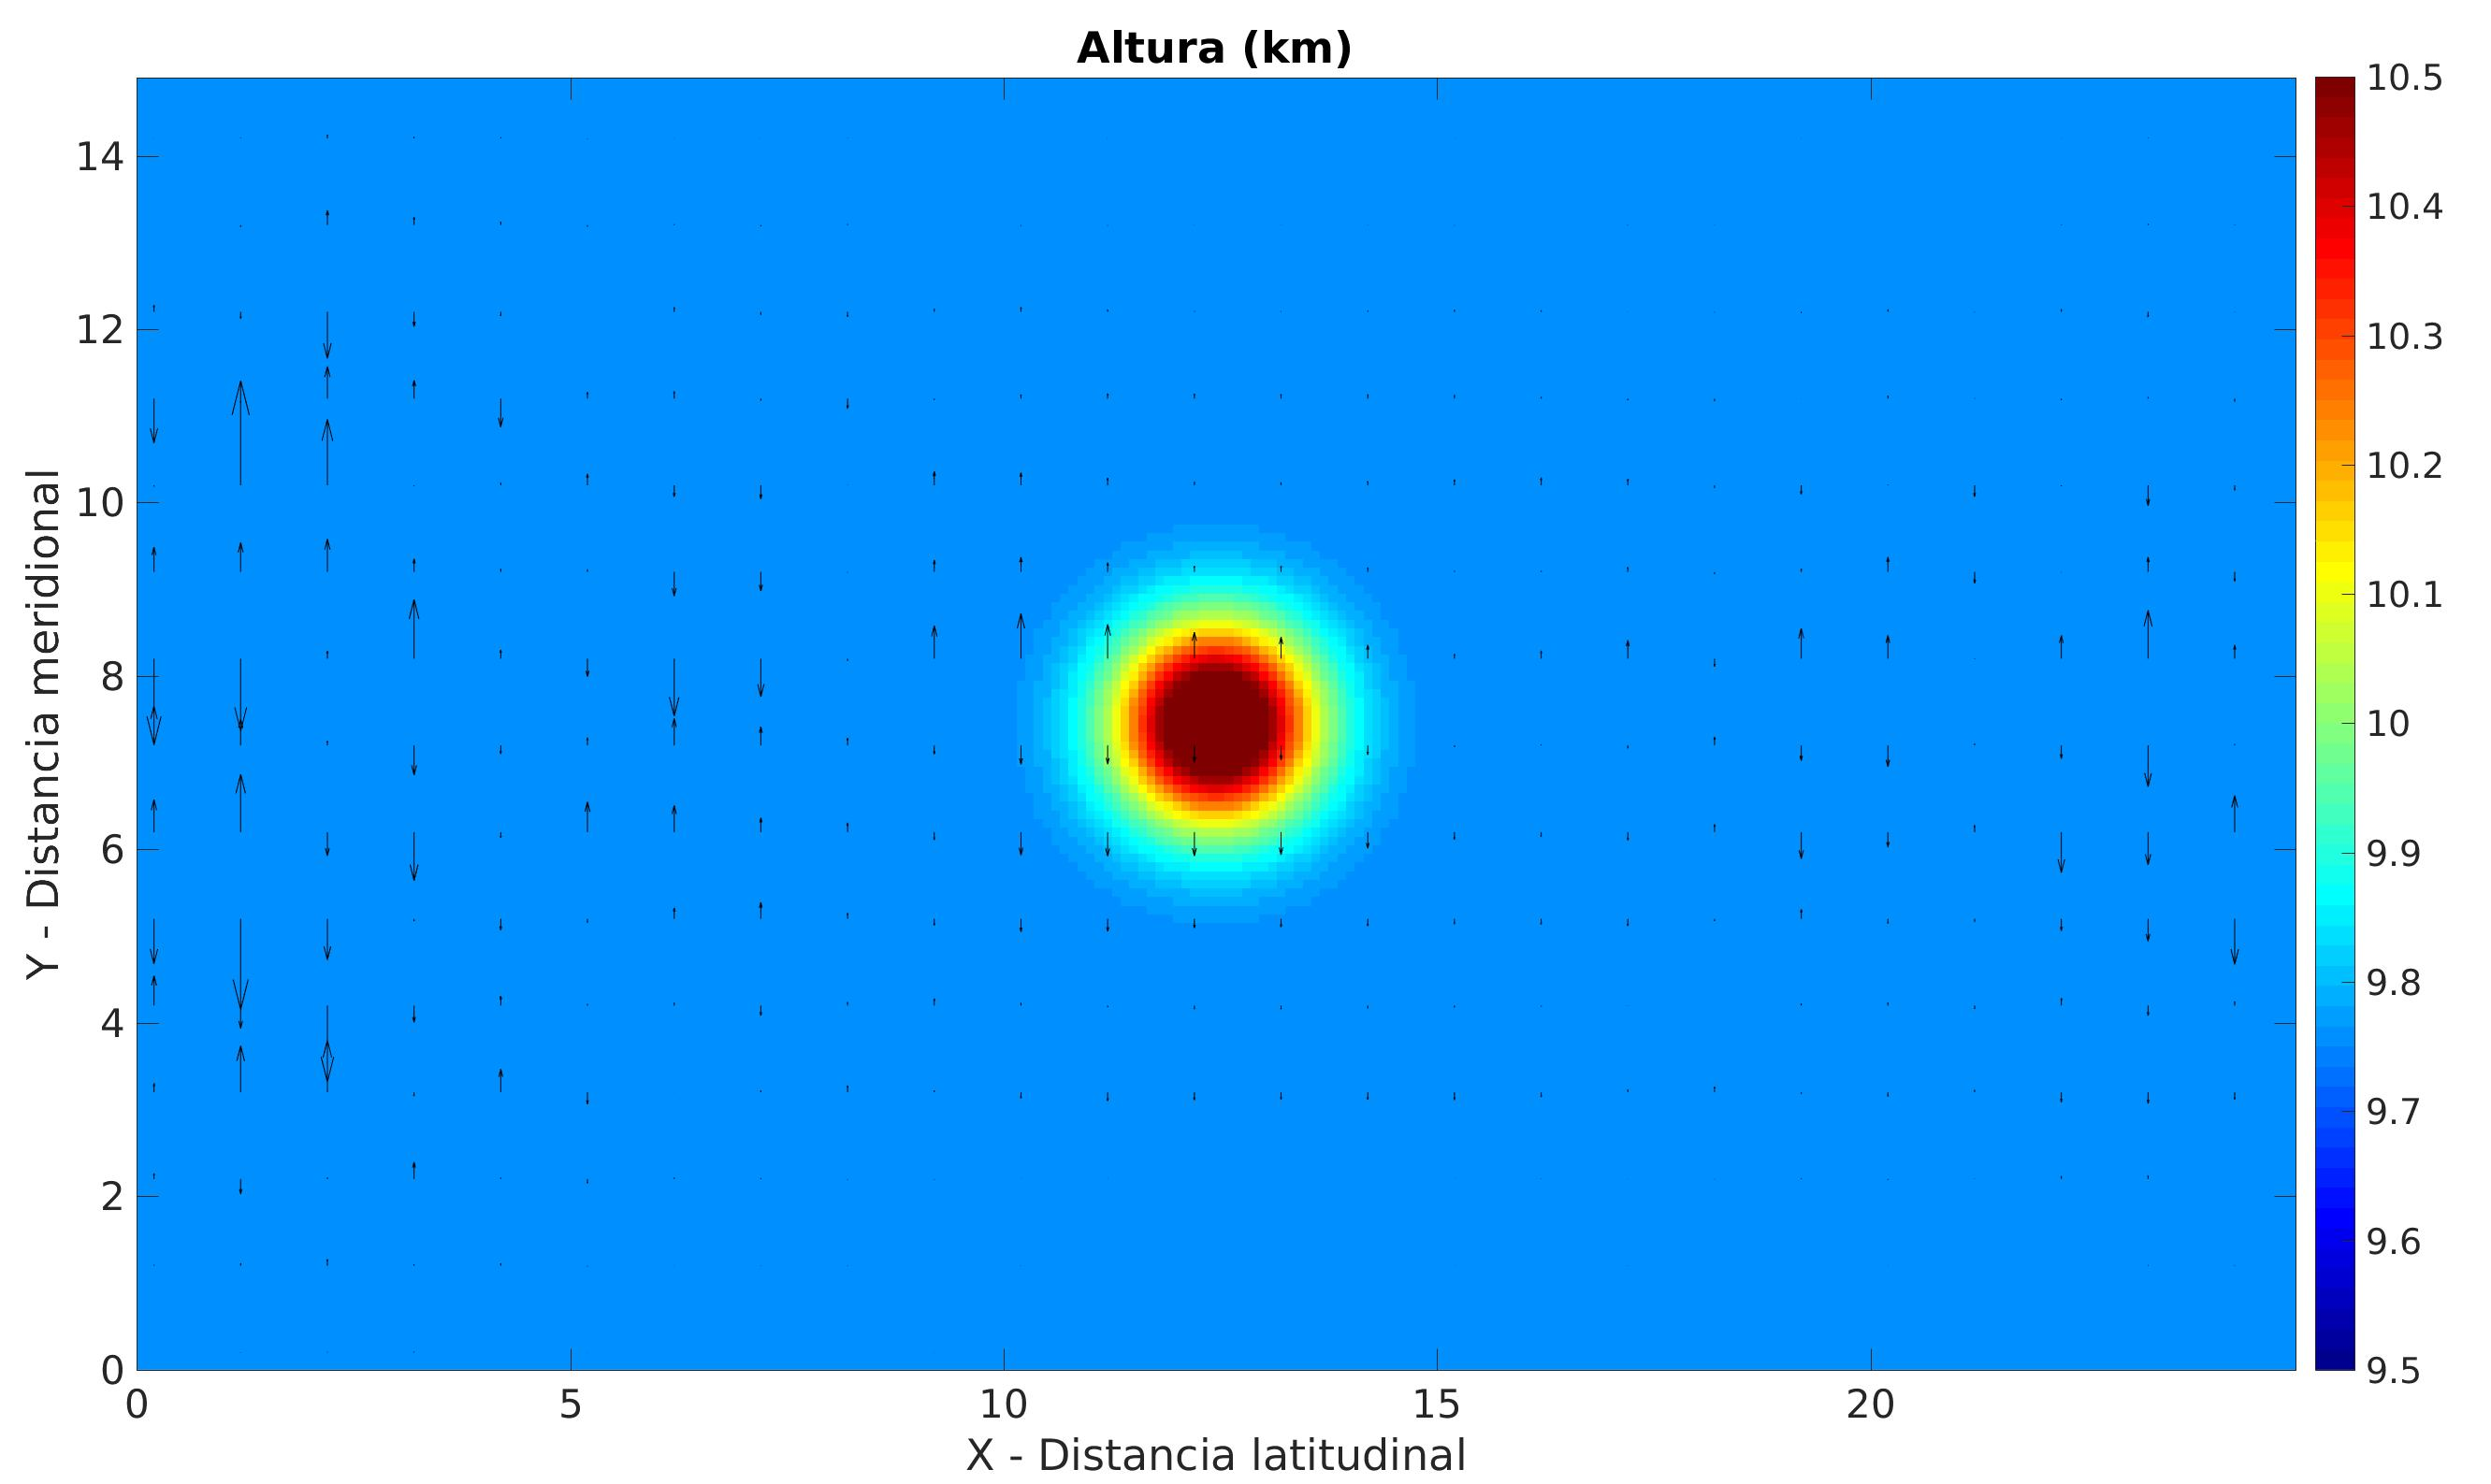
\includegraphics[scale=0.2]{k1.jpeg}
\caption{ }
\label{k1}
\end{minipage}
\hspace{0.1cm} 
\begin{minipage}[b]{0.5\linewidth}
\centering
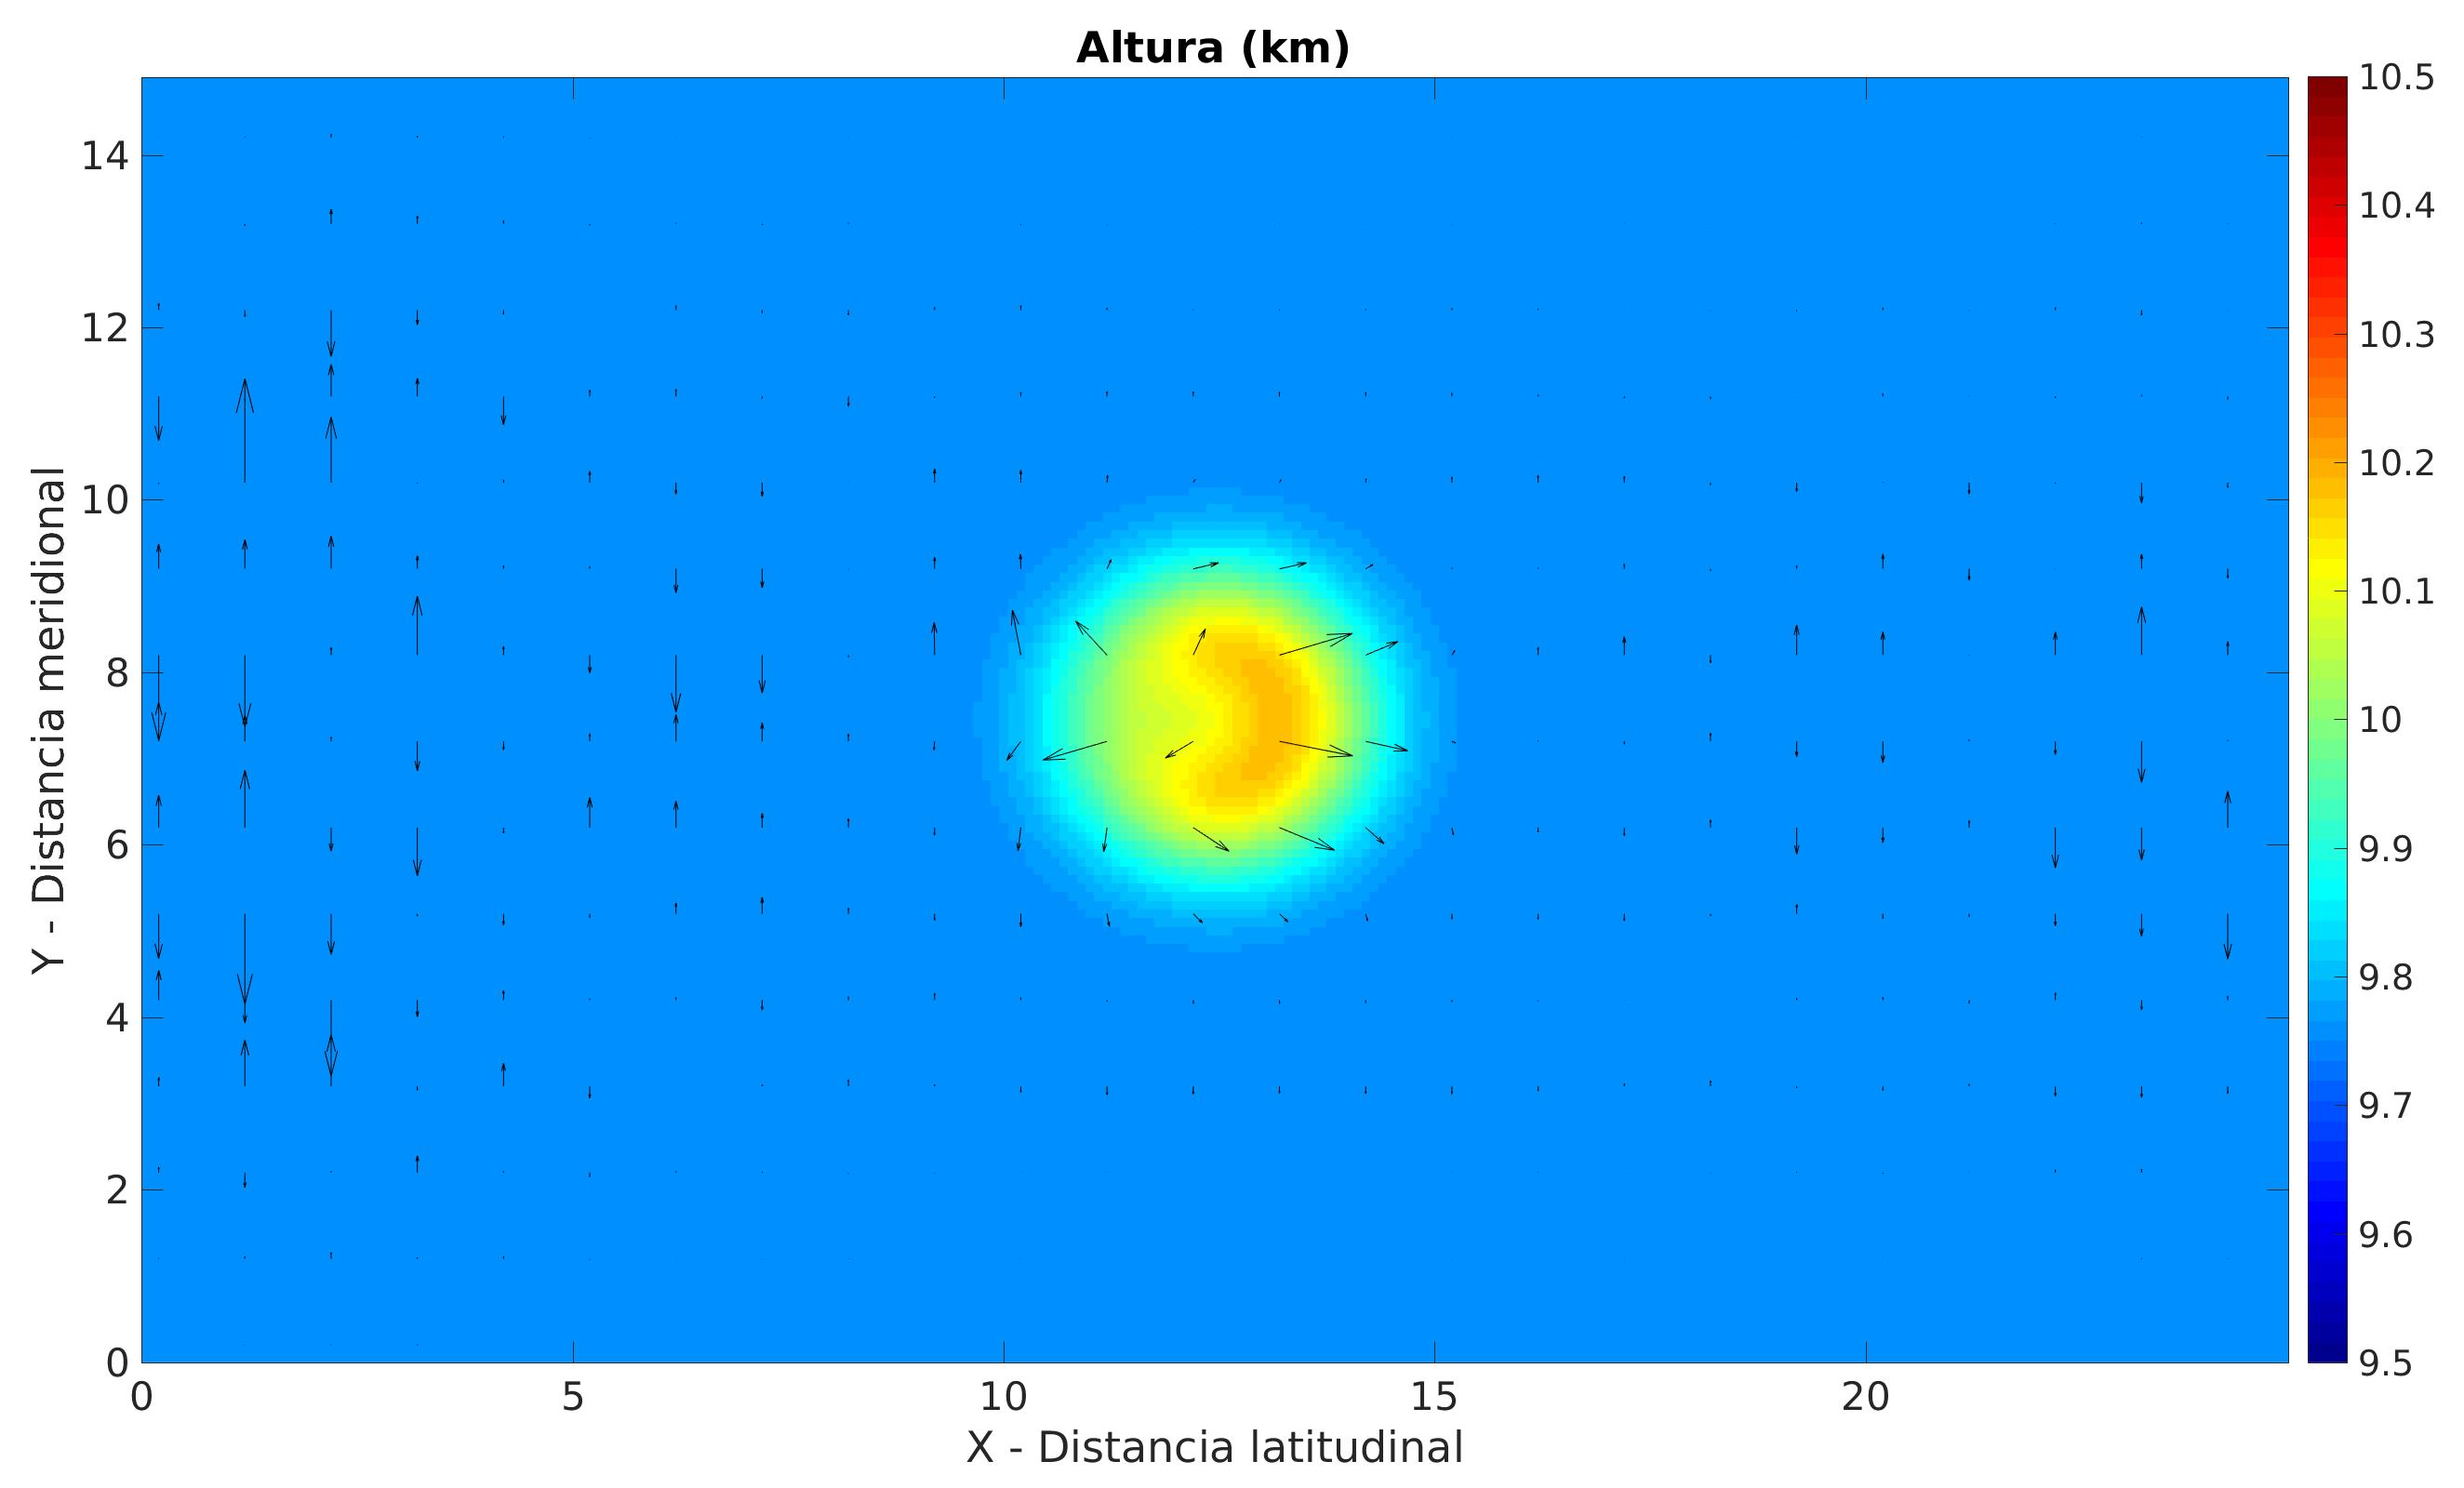
\includegraphics[scale=0.2]{k2.jpeg}
\caption{}
\label{k2}
\end{minipage}
\end{figure}


Lo que se observa ahora en las Figs. \ref{k3} y \ref{k4} es una onda que se propaga hacia el este sobre el ecuador denominada \texttt{onda de Kelvin} y dos ondas que viajan más lentamente hacia el oeste sobre los trópicos de Cáncer y de Capricornio denominadas \texttt{Ondas de Rossby}. La prueba sobre la dirección en que viajan las ondas está \href{http://meteo.fisica.edu.uy/Materias/oceanografia/teorico_oceanografia/cap7.pdf}{aquí} explícitamente.  


\begin{figure}[H]
\begin{minipage}[b]{0.5\linewidth} 
\centering
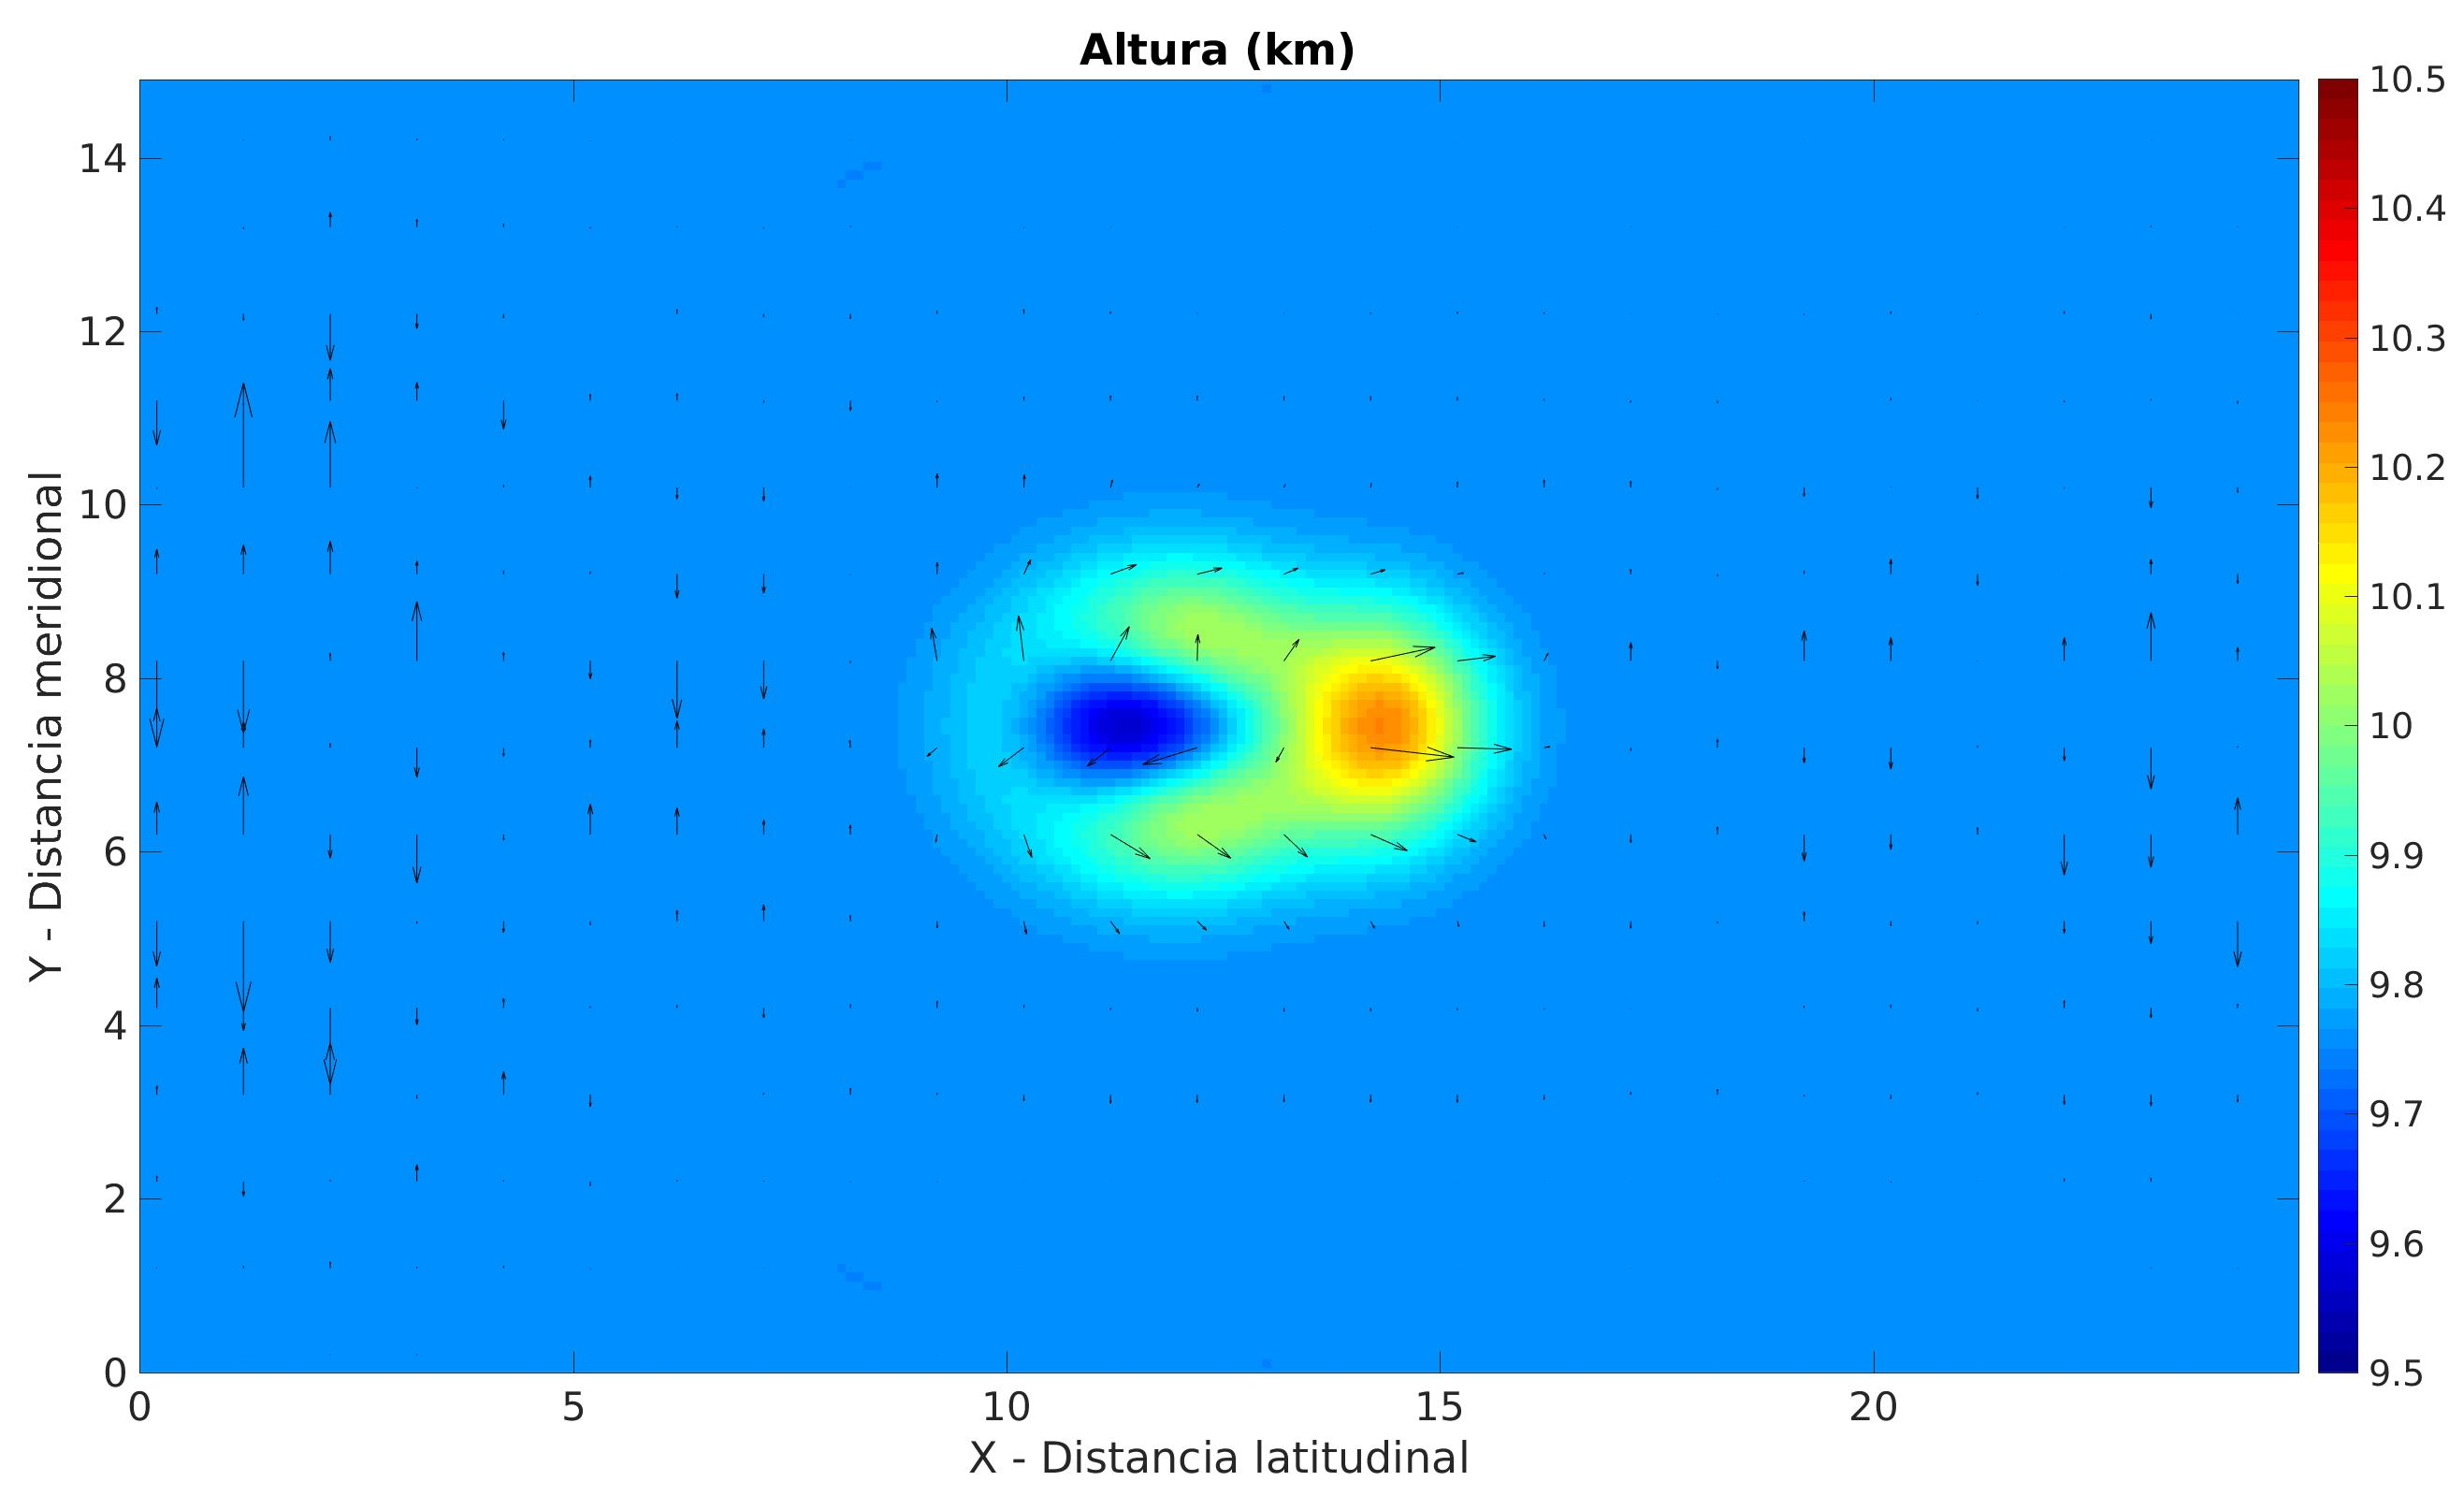
\includegraphics[scale=0.2]{k3.jpeg}
\caption{ }
\label{k3}
\end{minipage}
\hspace{0.1cm} 
\begin{minipage}[b]{0.5\linewidth}
\centering
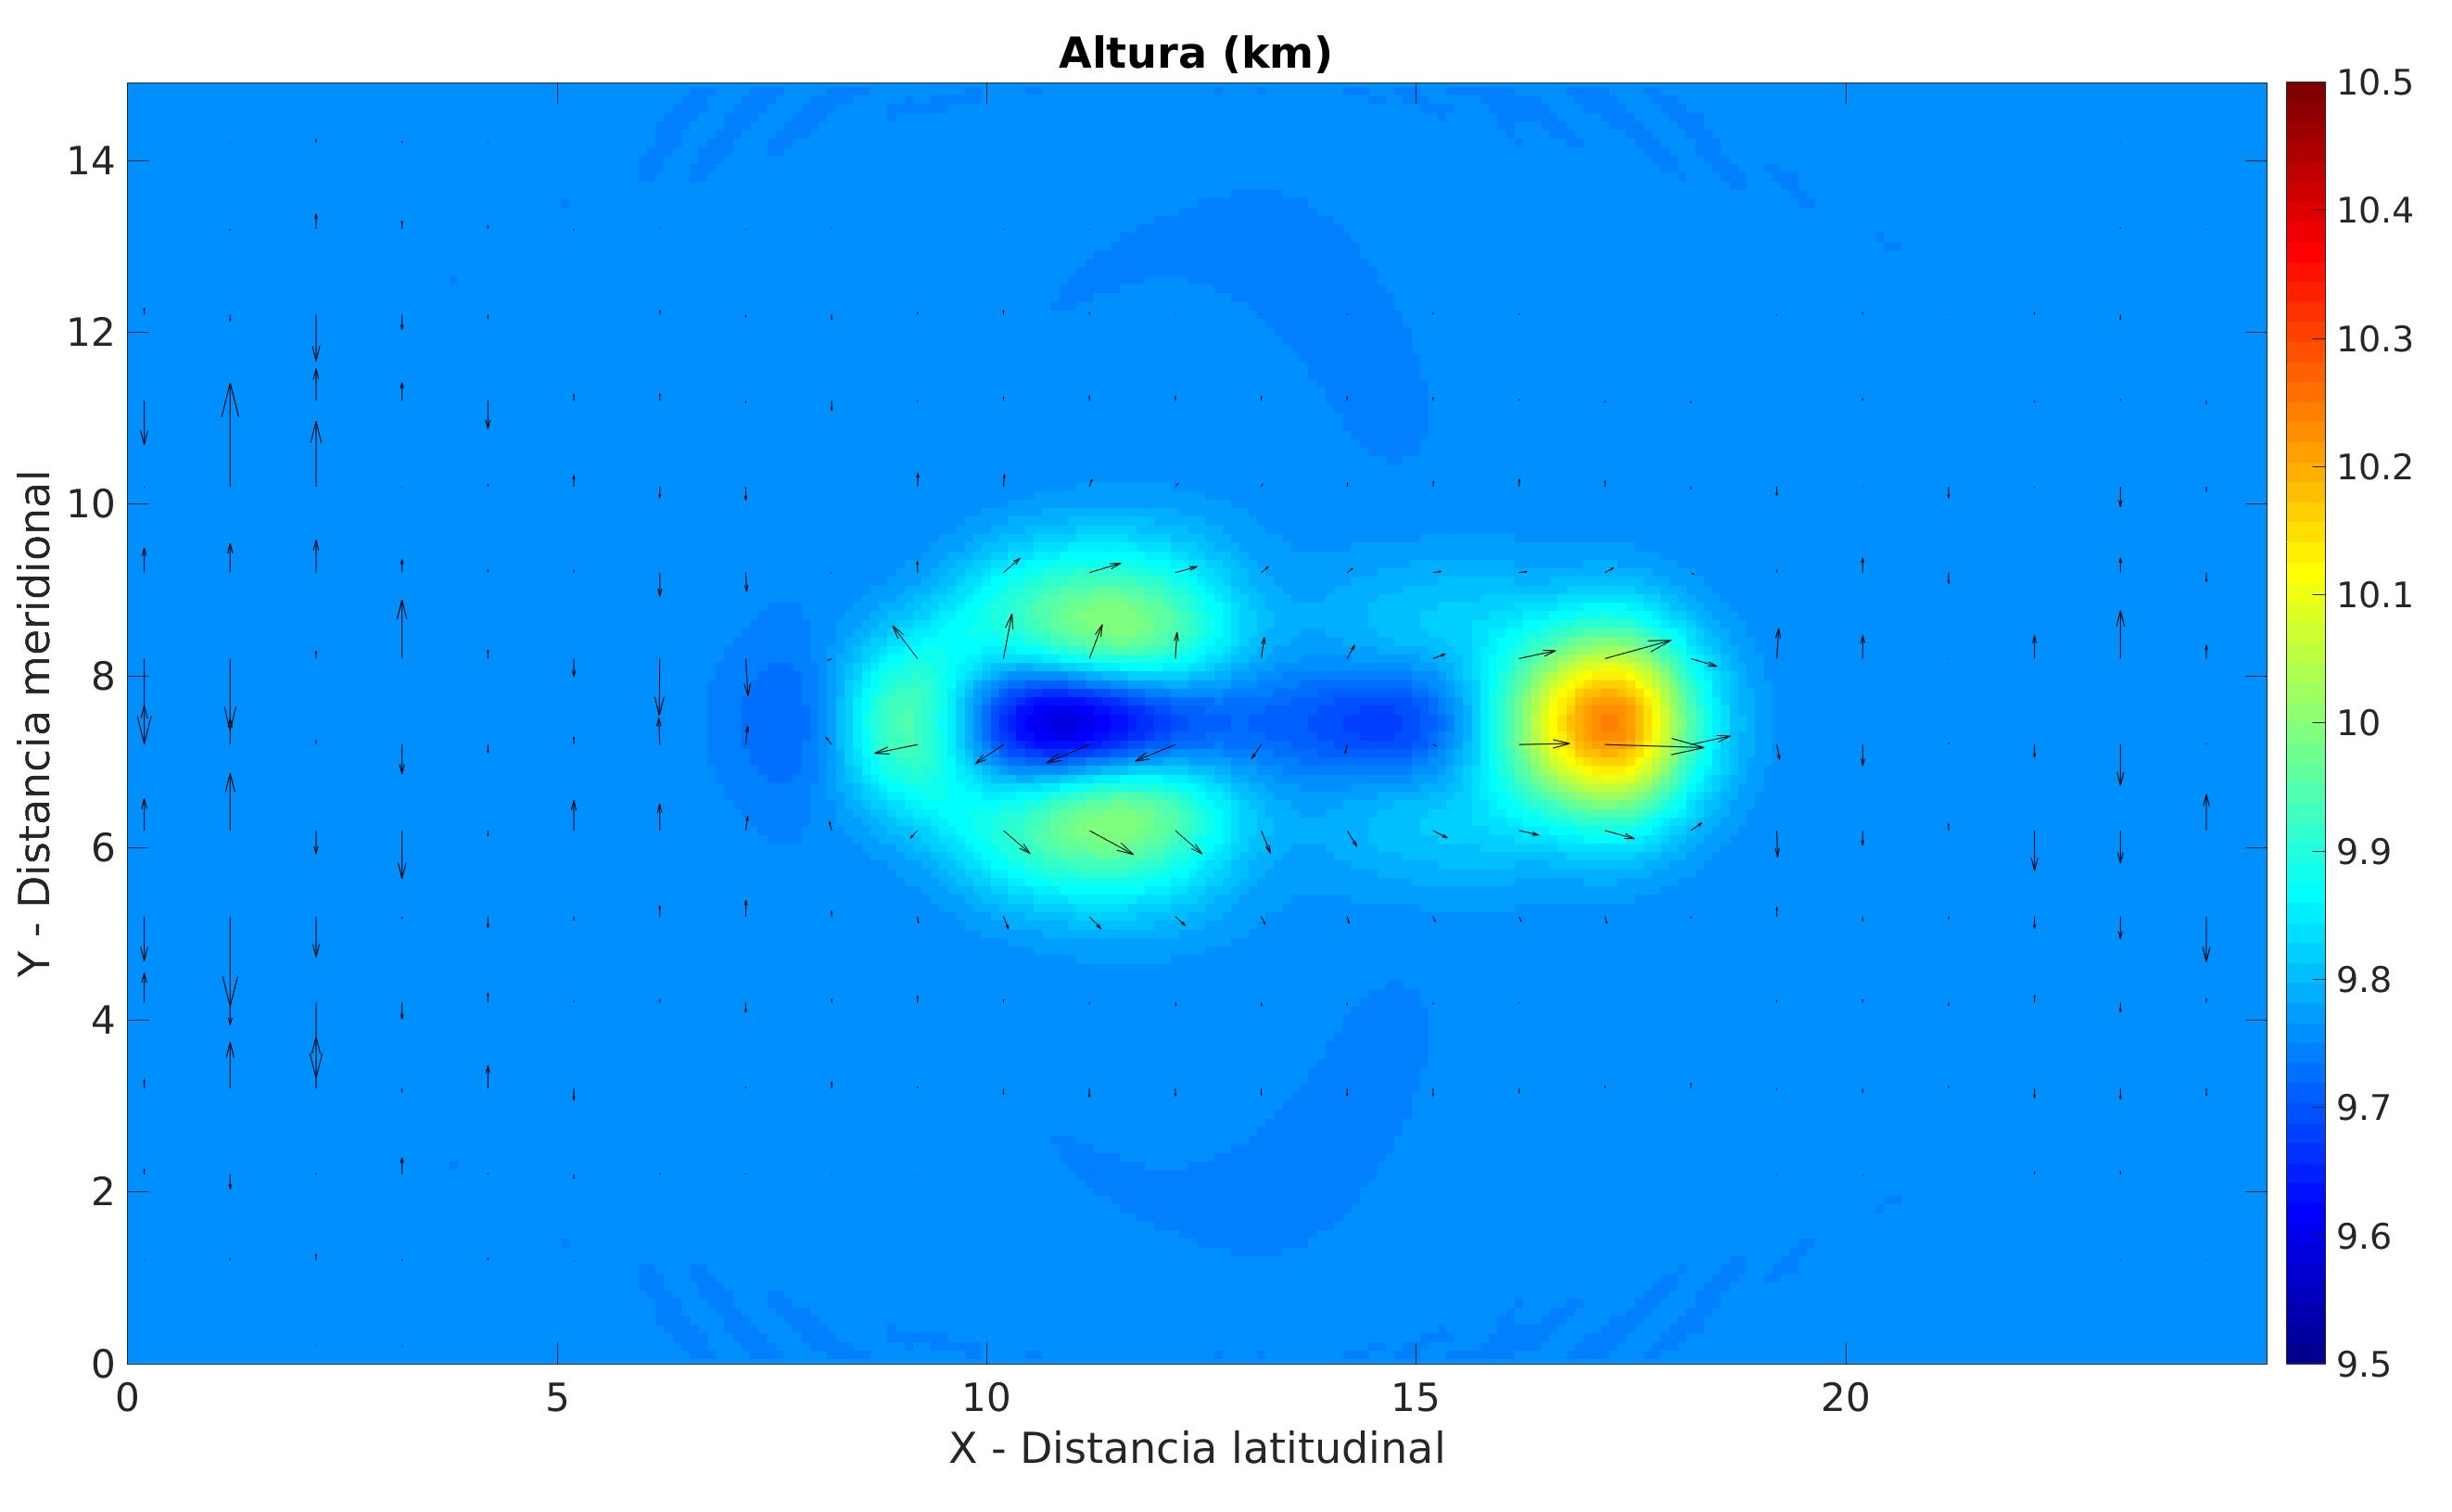
\includegraphics[scale=0.2]{k4.jpeg}
\caption{}
\label{k4}
\end{minipage}
\end{figure}

Simulación completa de la altura tipo película: \href{https://www.youtube.com/watch?v=iLz2mouRf5g&list=PLO4Ke9LzSkdFyMJ0r6OuJdeCk4Ys-RJ3t&index=3}{Altura - Ondas de Kelvin.}

El hecho de que la onda de Kelvin viaje más rápido que las ondas de Rossby se puede ver en la simulación del campo de velocidades $\xrightarrow{}$ \href{https://www.youtube.com/watch?v=8LDt5eNZDg0&list=PLO4Ke9LzSkdFyMJ0r6OuJdeCk4Ys-RJ3t&index=4}{Campo de velocidades - Ondas de Kelvin.}

Este experimento tiene como conclusión que cerca del ecuador la interacción de Coriolis es importante, hay que tenerla en cuenta y genera la separación de la onda de Kelvin de las ondas de Rossby. La onda de Kelvin se mueve hacia el este y las de Rossby que son ondas más pequeñas se mueven hacia el oeste. Este fenómeno puede ser observado en el fenómeno de El Niño que es introducido en las conclusiones a continuación.

\section{Conclusiones}

El estudio de las ondas de Kelvin permite analizar fenómenos muy importantes de la vida real como es el fenómeno de El Niño. 

Las ondas de Kelvin pueden ser formadas por ondas de Rossby en la frontera occidental del Pacífico. Las ondas de Kelvin viajan hacia el este con una velocidad típica de 2 a 3 metros por segundo por lo que si se formaron en el centro del Pacífico ecuatorial pueden demorarse entre un mes y medio y dos meses en llegar a la costa de América del Sur como se puede ver en la Fig. \ref{ni1}, de una simulación realizada por el Instituto Geofísico del Perú. Es por ello que resulta de fundamental importancia el  monitoreo y estudio de estas ondas para prevenir desastres provenientes de este tipo de fenómenos.


\begin{figure}[H]
\centering
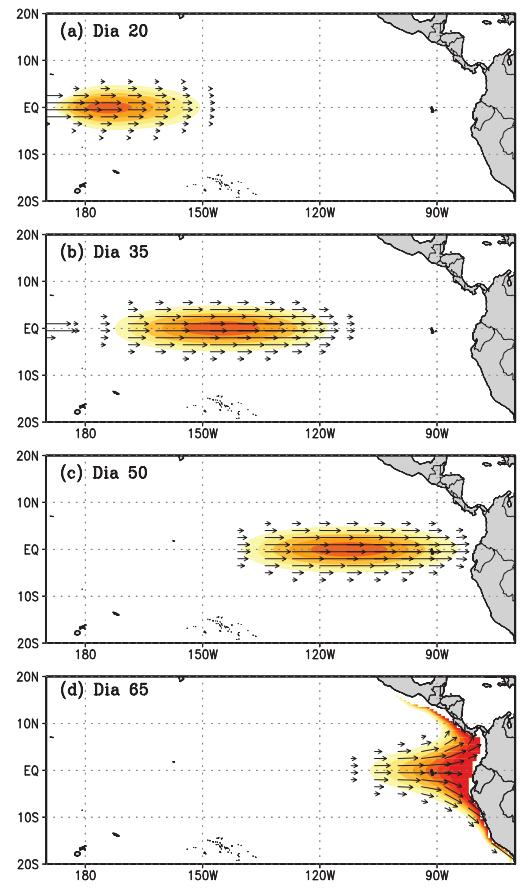
\includegraphics[scale=0.4]{ni1.jpeg}
\caption{Simulación tomada de \href{http://www.met.igp.gob.pe/publicaciones/2014/Boletin_El_Nino_201401.pdf}{aquí} de la propagación de una
onda de Kelvin ecuatorial forzada por un pulso de vientos del oeste ecuatorial centrado en $170^{\circ}E$ durante 30 días con un pico máximo de 9 m/s en el día 15.} \label{ni1}
\end{figure}

El fenómeno de El Niño puede ser explicado si se entiende como el océano tropical se ajusta a los cambios en los vientos \cite{nii1}. Este ajuste no es instantáneo, sino que involucra la propagación de ondas que llevan información desde una región a otra a lo largo del Pacífico tropical. Es en este proceso donde intervienen las ondas de Kelvin y de Rossby.


\section{Apéndice A: Derivaciones de las ecuaciones}
\subsection{Ecuación de Continuidad}

La ecuación de continuidad si la densidad $\rho$ es constante implica que la divergencia del campo de velocidades debe ser nula:
\begin{equation*}
    \frac{\partial \rho}{\partial t} = 0 \Rightarrow \vec{\nabla}    \cdot \vec{u} = 0
\end{equation*}
Sea $\vec{u} = (u,v,w)^{t}$, entonces:
\begin{equation*}
    \frac{\partial u}{\partial x} + \frac{\partial v}{\partial y} + \frac{\partial w}{\partial z} = 0
\end{equation*}

En este modelo se considera únicamente el flujo en 2 dimensiones. Sin embargo, existe una 3era dimensión que es la altura/profundidad del fluido $h$. Se asume que el movimiento vertical es el mismo a través de toda la profundidad del fluido por lo que se puede integrar la ecuación de continuidad en la coordenada $z$ entre $H$ y $h+H$:

\begin{equation}
    \int_{H}^{h+H}\frac{\partial u}{\partial x} dz + \int_{H}^{h+H}\frac{\partial v}{\partial y} dz + \int_{H}^{h+H}\frac{\partial w}{\partial z} dz = 0
\label{eq:c1}
\end{equation}

Para los primeros dos términos se aplica una técnica llamada en inglés \textit{differentiation under the integral sign} (Regla integral de Leibniz):

\begin{equation*}
        \int_{H}^{H + h(x,y)}\frac{\partial u}{\partial x} dz = \frac{\partial}{\partial x}\left(\int_{H}^{H + h(x,y)} u dz \right) - u(x,y) \hspace{0.08cm}\frac{\partial h}{\partial x}
\end{equation*}

Al evaluar la 3era integral de \ref{eq:c1}, queda $w(h+H) - w(H)$ y como $w(H) = 0$, esto es igual a la derivada total de $h$ respecto del tiempo, $\frac{d h}{dt} = \frac{\partial h}{\partial t} + u \frac{\partial h}{\partial x} + v \frac{\partial h}{\partial y}$. Entonces se recupera la ecuación de continuidad que es resuelta en el modelo de las SWE:

\begin{equation*}
\tcboxmath[colback=blue!25!white,colframe=blue, title=Ec. de Continuidad:]{
    \frac{\partial h}{\partial t} + \frac{\partial (u h)}{\partial x} + \frac{\partial (v h)}{\partial y} = 0 }
\end{equation*}

\subsection{Ecuación para la presión}

Se asume que el fluido está en condiciones de un balance hidrostático:

\begin{equation*}
    \frac{\partial P}{\partial z} = - \rho g
\end{equation*}
con $\rho$ constante.

La ecuación hidrostática con densidad constante implica que podemos describir la presión en función de la altura $z$:

\begin{equation*}
    P(z) = - \rho g (z - H) + P_{s}(x,y,t)
\end{equation*}

donde H es la altura de la orografía, es decir la altura de la superficie sólida sobre la que se apoya el fluido como por ejemplo las montañas. Imponiendo la condición de contorno $P(z = h + H) = 0$ se determina $P_{s}$ y se obtiene finalmente:

\begin{equation}
P(z) = - \rho g (z - (H + h))    
\label{eq:pp}
\end{equation}

\subsubsection{Ecuaciones de Navier-Stokes en 2D}
Las ecuaciones de Navier-Stokes en 2D son las ecuaciones no conservativas del momento en el plano x-y:

\begin{equation}
    \frac{\partial u}{\partial t} + u \frac{\partial u}{\partial x} + v \frac{\partial u}{\partial y} = f v - \frac{1}{\rho} \frac{\partial P}{\partial x}
    \label{nc1}
\end{equation}

\begin{equation}
        \frac{\partial v}{\partial t} + u \frac{\partial v}{\partial x} + v \frac{\partial v}{\partial y} = -f u - \frac{1}{\rho} \frac{\partial P}{\partial y}
        \label{nc2}
\end{equation}

Se observa que las Ecs. \ref{nc1} y \ref{nc2} contienen varios términos no lineales, que no pueden ser discretizados fácilmente con algún esquema numérico.

Si se utiliza la Ec. \ref{eq:pp} se obtiene que el RHS de las Ecs. \ref{nc1} y \ref{nc2} puede ser reemplazado por:

\begin{equation*}
    -\frac{1}{\rho} \frac{\partial P}{\partial x} = - g \frac{\partial (h + H)}{\partial x}
\end{equation*}

\begin{equation*}
        -\frac{1}{\rho} \frac{\partial P}{\partial y} = - g \frac{\partial (h + H)}{\partial y}
\end{equation*}

Para obtener las Ecs. \ref{cons1} y \ref{cons2}, utilizamos las ecuaciones no conservativas del momento horizontal \ref{nc1} y \ref{nc2} junto a la ecuación de continuidad para derivar las ecuaciones conservativas del momento horizontal.

En primer lugar se multiplica por $h$ a las Ecs. \ref{nc1} y \ref{nc2}:

\begin{equation}
    h \frac{\partial u}{\partial t} + h u \frac{\partial u}{\partial x} + h v \frac{\partial u}{\partial y} = f h v - h g \frac{\partial (h + H)}{\partial x}
    \label{u1}
\end{equation}

\begin{equation}
    h \frac{\partial v}{\partial t} + h u \frac{\partial v}{\partial x} + h v \frac{\partial v}{\partial y} = - f h u - h g \frac{\partial (h + H)}{\partial y}
    \label{v1}
\end{equation}


Luego se suma el producto de $u$ y la ecuación de continuidad a la Ec. \ref{u1} por un lado y por el otro lado se suma el producto de $v$ y la ecuación de continuidad a la Ec. \ref{v1}. Para el caso de $u$ esto resulta:

\begin{equation*}
    h \frac{\partial u}{\partial t} + u \frac{\partial h}{\partial t} + u \frac{\partial (h u)}{\partial x} + u \frac{\partial (h v)}{\partial y} + h u \frac{\partial u}{\partial x} + h v \frac{\partial u}{\partial y} = f h v - h g \frac{\partial (h +H)}{\partial x}
\end{equation*}

Usando la regla de la derivada del producto se obtienen las ecuaciones de conservación del momento de las SWE, Ecs. \ref{cons1} y \ref{cons2}:


\begin{equation*}
\tcboxmath{\frac{\partial u h}{\partial t} + \frac{\partial (u^{2} h + g h^{2}/2)}{\partial x} + \frac{\partial (u v h)}{\partial y} = h \left(f v - g \frac{\partial H}{\partial x}\right)}
\end{equation*}

\begin{equation*}
\tcboxmath{    \frac{\partial v h}{\partial t} + \frac{\partial (u v h)}{\partial x} + \frac{\partial (v^{2} h + g h^{2}/2)}{\partial y}  = h \left(-f u - g \frac{\partial H}{\partial y}\right)}
\end{equation*}

\section{Apéndice B: Derivación del esquema numérico de Lax-Wendroff}

Consideremos la ecuación 1D de convección:
\begin{center}
\begin{equation*}
\dfrac{\partial u}{\partial t} + c \dfrac{\partial u}{\partial x} = 0
\end{equation*}
\end{center}
La receta para obtener el esquema de Lax-Wendroff es:
\begin{enumerate}
    \item Expansión de Taylor en el tiempo alrededor de $u_{i}^{n}$ y nos quedamos hasta $\order{{\Delta t}^{2}}$.
    \item Se deriva respecto del tiempo la ecuación 1D de convección $u_{t} + c u_{x}$, resultando $u_{tt} = - c (u_{t})_{x}$. En esta última expresión se reemplaza la ecuación 1D de convección obteniéndose $u_{tt} = c^{2} u_{xx}$ $\xrightarrow{}$ se lo reemplaza en la expansión de Taylor del paso 1.
    \item Se discretizan las derivadas espaciales utilizando diferencias centradas.
\end{enumerate}

De esta forma se obtiene el esquema de Lax-Wendroff:

\begin{equation*}
    u(x_{i},t_{n+1})=u_{i}^{n+1}=u_{i}^{n}-\dfrac{c\Delta t}{2\Delta x}(u_{i+1}^{n}-u_{i-1}^{n})+\dfrac{c^2\Delta t^2}{2\Delta x^2}(u_{i+1}^{n}-2u_{i}^{n}+u_{i-1}^{n})
\end{equation*}
%donde $t_{n}$ representa el $n$-ésimo paso temporal y $x_{i}$ representa la i-ésima cuadrícula.

El error de truncado es de orden $\mathcal{O}({\Delta t}^{2} + {\Delta x}^{2})$ por lo que se dice que el método tiene una exactitud de 2do orden.

Al mismo tiempo, este método puede ser modificado a uno de dos pasos en donde cada paso individual está centrado tanto en el tiempo como en el espacio:

\begin{equation*}
\tcboxmath[title=Paso 1 - Lax-Friedrichs]{\dfrac{u_{i+\frac{1}{2}}^{n+\frac{1}{2}}-\dfrac{1}{2}(u_{i+1}^n+u_{i}^n)}{\dfrac{1}{2}\Delta t}=-c\left(\dfrac{u_{i+1}^n-u_{i}^n}{\Delta x}\right)}
\end{equation*}

\begin{equation*}
\tcboxmath[title=Paso 2 - Leapfrog]{\dfrac{u_{i-\frac{1}{2}}^{n+\frac{1}{2}}-\dfrac{1}{2}(u_{i}^n+u_{i-1}^n)}{\dfrac{1}{2}\Delta t}=-c\left(\dfrac{u_{i}^n-u_{i-1}^n}{\Delta x}\right)}
\end{equation*}

En el segundo paso, $u_{i}^{n+1}$ sale de computar:

\begin{equation*}
    \dfrac{u_{j}^{n+1}-u_{j}^{n}}{\Delta t}=-c\left(\dfrac{u_{j+\frac{1}{2}}^{n+\frac{1}{2}}-u_{j-\frac{1}{2}}^{n+\frac{1}{2}}}{\Delta x}\right)
\end{equation*}

El stencil en 1D del esquema se muestra en la Fig. \ref{lwaf}.

\begin{figure}[H]
\centering
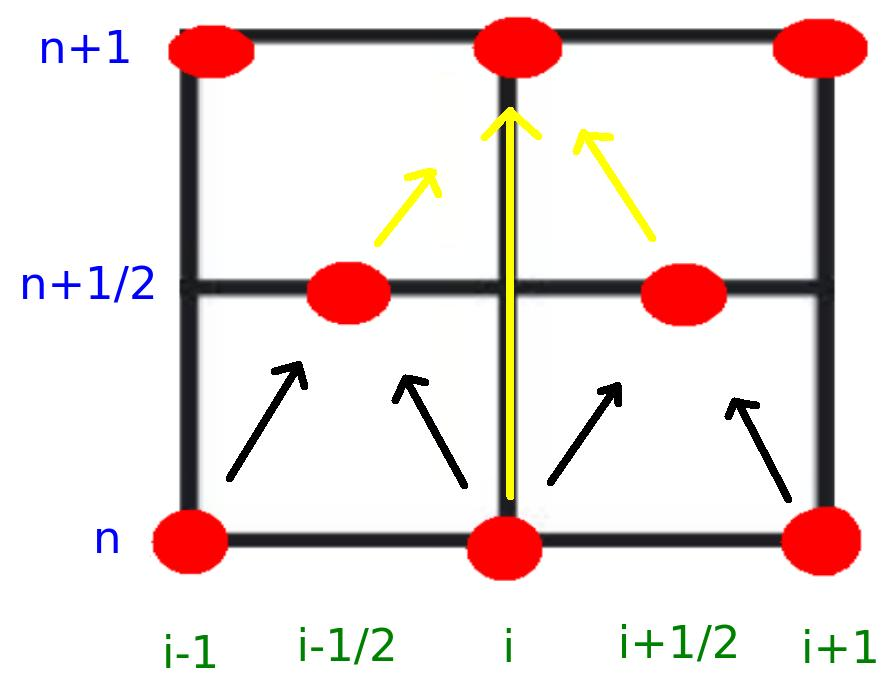
\includegraphics[scale=0.7]{lwa.jpeg}
\caption{Stencil en 1D del esquema numérico de Lax-Wendroff.} \label{lwaf}
\end{figure}


Si se extiende el esquema de dos pasos a 2D, para la ecuación de convección en 2D, se obtiene:

\begin{equation}
    \tcboxmath[]{u_{i+\frac{1}{2},j}^{n+\frac{1}{2}} = \dfrac{1}{2}(u_{i+1,j}^n+u_{i,j}^n)-\dfrac{1}{2}\dfrac{c\Delta t}{\Delta x}(u_{i+1,j}^n-u_{i,j}^n)}
\label{esq1}
\end{equation}

\begin{equation}
    \tcboxmath[]{u_{i,j+\frac{1}{2}}^{n+\frac{1}{2}} = \dfrac{1}{2}(u_{i,j+1}^n+u_{i,j}^n)-\dfrac{1}{2}\dfrac{c\Delta t}{\Delta y}(u_{i,j+1}^n-u_{i,j}^n)}
\label{esq2}
\end{equation}

\begin{equation}
    \tcboxmath[]{u_{i,j}^{n+1}=u_{i,j}^n-c \Delta t \left[  \dfrac{u_{i+\frac{1}{2},j}^{n+\frac{1}{2}}-u_{i-\frac{1}{2},j}^{n+\frac{1}{2}}}{\Delta x} +   \dfrac{u_{i,j+\frac{1}{2}}^{n+\frac{1}{2}}-u_{i,j-\frac{1}{2}}^{n+\frac{1}{2}}}{\Delta y}  \right]}
\label{esq3}
\end{equation}

Si tenemos un término fuente / sumidero, sólo tiene que ser agregado en el RHS de la Ec. \ref{esq3}:

\begin{equation}
\tcboxmath[]{u_{i,j}^{n+1}=u_{i,j}^n-c \Delta t \left[  \dfrac{u_{i+\frac{1}{2},j}^{n+\frac{1}{2}}-u_{i-\frac{1}{2},j}^{n+\frac{1}{2}}}{\Delta x} +   \dfrac{u_{i,j+\frac{1}{2}}^{n+\frac{1}{2}}-u_{i,j-\frac{1}{2}}^{n+\frac{1}{2}}}{\Delta y}  \right] + S_{i,j}^{n+\frac{1}{2}} \Delta t}
\label{esq4}
\end{equation}


\newpage
\phantomsection
\addcontentsline{toc}{section}{6.\hspace{0.1cm} Referencias} 
\begin{thebibliography}{0}
    \bibitem{Vallis} \textsc{Vallis, G. K.} (2006) \textit{Atmospheric and Oceanic Fluid Dynamics. Cambridge University Press.}
  \bibitem{nii1} \textsc{Pizarro, O. y A. Montecinos} (2005) \textit{El Niño y la Oscilación del Sur, Cap. 7 en Biología Marina y Oceanografía: Conceptos y Procesos. Ed. C. Werlinger, Universidad de Concepción, Concepción}
  \bibitem{dds} \textsc{James R. Holton} (2004) \textit{An Introduction to Dynamic Meterology} Elsevier, Academic Press.
 \bibitem{Barba} \textsc{Barba L.} (2014) \textit{12 steps to Navier-Stokes equations} \url{https://www.youtube.com/watch?v=cDy5XGOokBY&list=PL30F4C5ABCE62CB61}
  \bibitem{Weller} \textsc{Weller H.} (2015) \textit{MPECDT numerics course} \url{https://www.youtube.com/watch?v=gnqFGE5G9rY&list=PLEG35I51CH7W6bOW3UbkjHRSQfdSk3TRh}
 
 
\end{thebibliography}

















\end{document}





